\documentclass[1p]{elsarticle_modified}
%\bibliographystyle{elsarticle-num}

%\usepackage[colorlinks]{hyperref}
%\usepackage{abbrmath_seonhwa} %\Abb, \Ascr, \Acal ,\Abf, \Afrak
\usepackage{amsfonts}
\usepackage{amssymb}
\usepackage{amsmath}
\usepackage{amsthm}
\usepackage{scalefnt}
\usepackage{amsbsy}
\usepackage{kotex}
\usepackage{caption}
\usepackage{subfig}
\usepackage{color}
\usepackage{graphicx}
\usepackage{xcolor} %% white, black, red, green, blue, cyan, magenta, yellow
\usepackage{float}
\usepackage{setspace}
\usepackage{hyperref}

\usepackage{tikz}
\usetikzlibrary{arrows}

\usepackage{multirow}
\usepackage{array} % fixed length table
\usepackage{hhline}

%%%%%%%%%%%%%%%%%%%%%
\makeatletter
\renewcommand*\env@matrix[1][\arraystretch]{%
	\edef\arraystretch{#1}%
	\hskip -\arraycolsep
	\let\@ifnextchar\new@ifnextchar
	\array{*\c@MaxMatrixCols c}}
\makeatother %https://tex.stackexchange.com/questions/14071/how-can-i-increase-the-line-spacing-in-a-matrix
%%%%%%%%%%%%%%%

\usepackage[normalem]{ulem}

\newcommand{\msout}[1]{\ifmmode\text{\sout{\ensuremath{#1}}}\else\sout{#1}\fi}
%SOURCE: \msout is \stkout macro in https://tex.stackexchange.com/questions/20609/strikeout-in-math-mode

\newcommand{\cancel}[1]{
	\ifmmode
	{\color{red}\msout{#1}}
	\else
	{\color{red}\sout{#1}}
	\fi
}

\newcommand{\add}[1]{
	{\color{blue}\uwave{#1}}
}

\newcommand{\replace}[2]{
	\ifmmode
	{\color{red}\msout{#1}}{\color{blue}\uwave{#2}}
	\else
	{\color{red}\sout{#1}}{\color{blue}\uwave{#2}}
	\fi
}

\newcommand{\Sol}{\mathcal{S}} %segment
\newcommand{\D}{D} %diagram
\newcommand{\A}{\mathcal{A}} %arc


%%%%%%%%%%%%%%%%%%%%%%%%%%%%%5 test

\def\sl{\operatorname{\textup{SL}}(2,\Cbb)}
\def\psl{\operatorname{\textup{PSL}}(2,\Cbb)}
\def\quan{\mkern 1mu \triangleright \mkern 1mu}

\theoremstyle{definition}
\newtheorem{thm}{Theorem}[section]
\newtheorem{prop}[thm]{Proposition}
\newtheorem{lem}[thm]{Lemma}
\newtheorem{ques}[thm]{Question}
\newtheorem{cor}[thm]{Corollary}
\newtheorem{defn}[thm]{Definition}
\newtheorem{exam}[thm]{Example}
\newtheorem{rmk}[thm]{Remark}
\newtheorem{alg}[thm]{Algorithm}

\newcommand{\I}{\sqrt{-1}}
\begin{document}

%\begin{frontmatter}
%
%\title{Boundary parabolic representations of knots up to 8 crossings}
%
%%% Group authors per affiliation:
%\author{Yunhi Cho} 
%\address{Department of Mathematics, University of Seoul, Seoul, Korea}
%\ead{yhcho@uos.ac.kr}
%
%
%\author{Seonhwa Kim} %\fnref{s_kim}}
%\address{Center for Geometry and Physics, Institute for Basic Science, Pohang, 37673, Korea}
%\ead{ryeona17@ibs.re.kr}
%
%\author{Hyuk Kim}
%\address{Department of Mathematical Sciences, Seoul National University, Seoul 08826, Korea}
%\ead{hyukkim@snu.ac.kr}
%
%\author{Seokbeom Yoon}
%\address{Department of Mathematical Sciences, Seoul National University, Seoul, 08826,  Korea}
%\ead{sbyoon15@snu.ac.kr}
%
%\begin{abstract}
%We find all boundary parabolic representation of knots up to 8 crossings.
%
%\end{abstract}
%\begin{keyword}
%    \MSC[2010] 57M25 
%\end{keyword}
%
%\end{frontmatter}

%\linenumbers
%\tableofcontents
%
\newcommand\colored[1]{\textcolor{white}{\rule[-0.35ex]{0.8em}{1.4ex}}\kern-0.8em\color{red} #1}%
%\newcommand\colored[1]{\textcolor{white}{ #1}\kern-2.17ex	\textcolor{white}{ #1}\kern-1.81ex	\textcolor{white}{ #1}\kern-2.15ex\color{red}#1	}

{\Large $\underline{12a_{1053}~(K12a_{1053})}$}

\setlength{\tabcolsep}{10pt}
\renewcommand{\arraystretch}{1.6}
\vspace{1cm}\begin{tabular}{m{100pt}>{\centering\arraybackslash}m{274pt}}
\multirow{5}{120pt}{
	\centering
	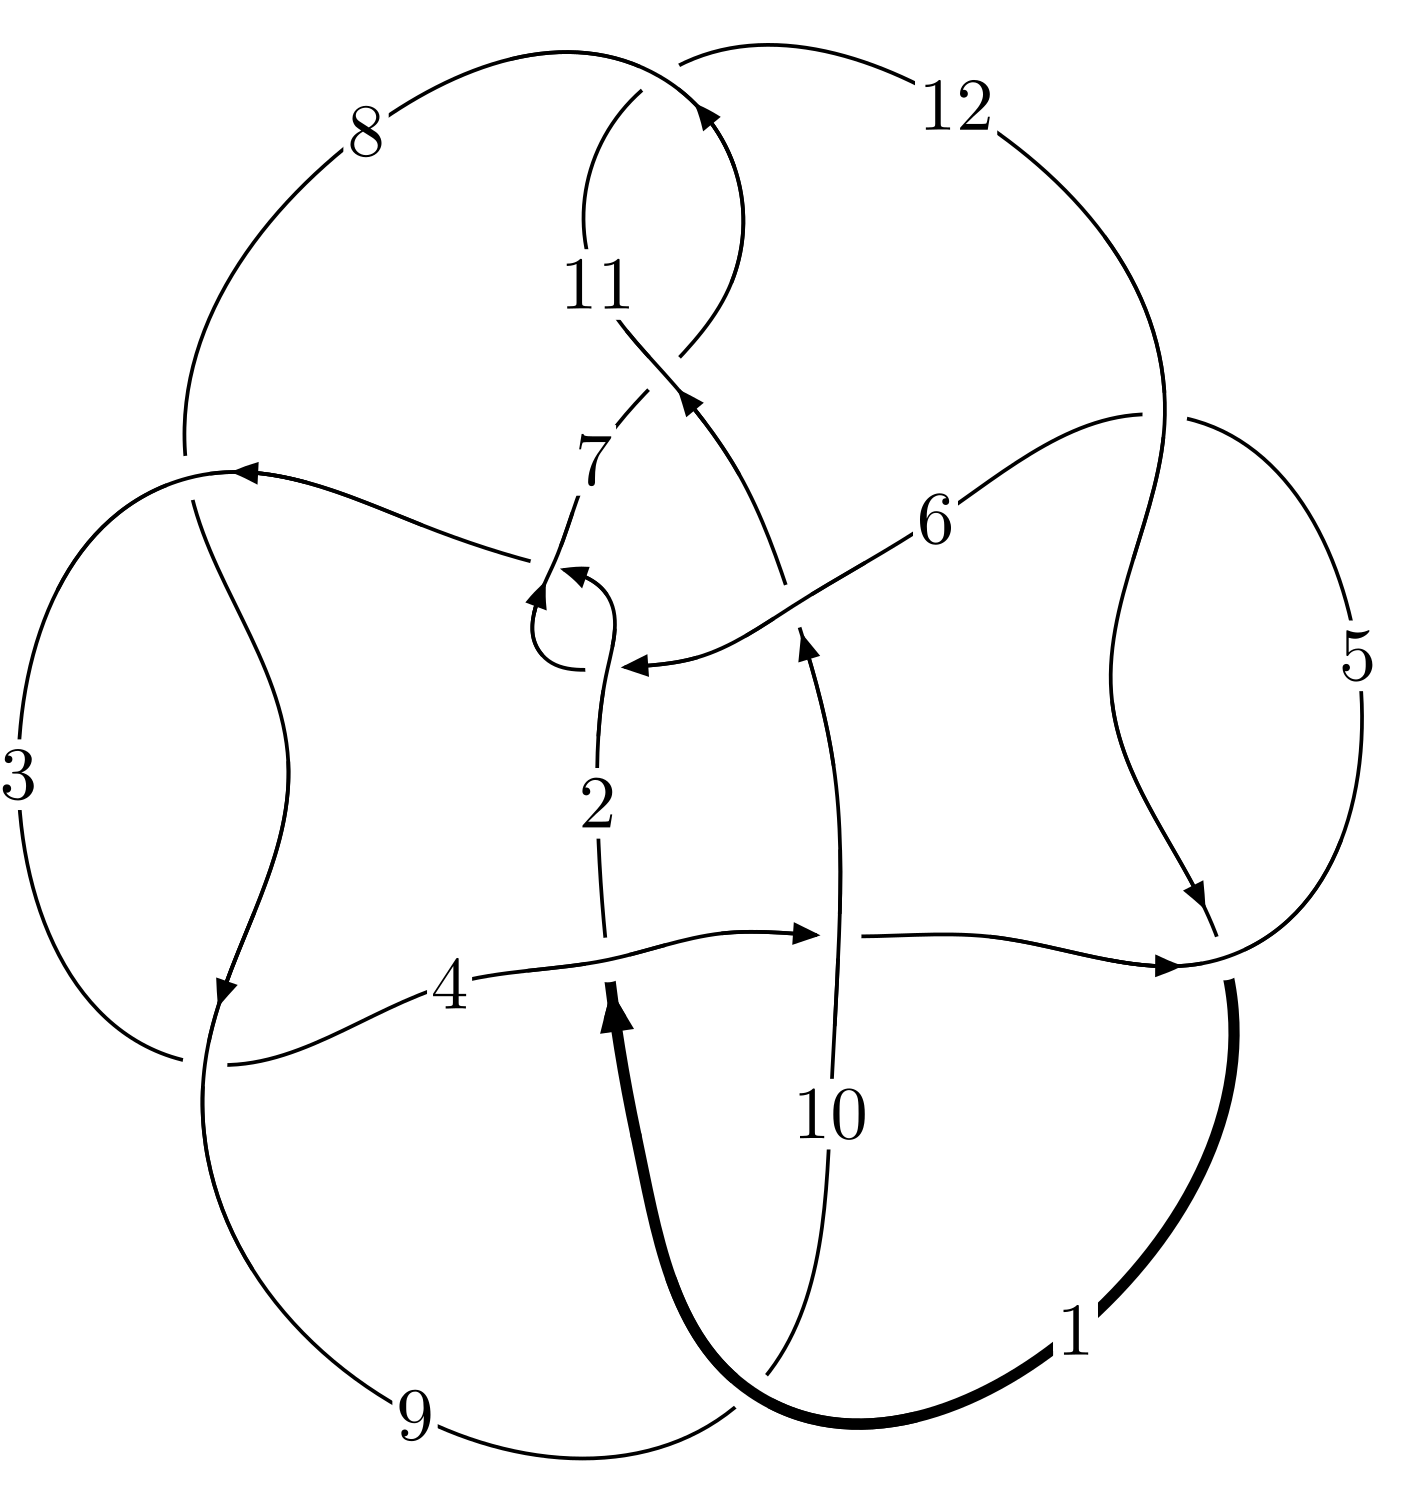
\includegraphics[width=112pt]{../../../GIT/diagram.site/Diagrams/png/1854_12a_1053.png}\\
\ \ \ A knot diagram\footnotemark}&
\allowdisplaybreaks
\textbf{Linearized knot diagam} \\
\cline{2-2}
 &
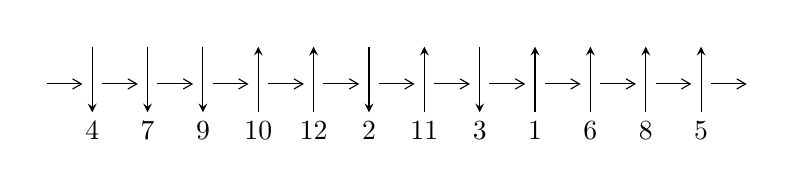
\begin{tikzpicture}[x=20pt, y=17pt]
	% nodes
	\node (C0) at (0, 0) {};
	\node (C1) at (1, 0) {};
	\node (C1U) at (1, +1) {};
	\node (C1D) at (1, -1) {4};

	\node (C2) at (2, 0) {};
	\node (C2U) at (2, +1) {};
	\node (C2D) at (2, -1) {7};

	\node (C3) at (3, 0) {};
	\node (C3U) at (3, +1) {};
	\node (C3D) at (3, -1) {9};

	\node (C4) at (4, 0) {};
	\node (C4U) at (4, +1) {};
	\node (C4D) at (4, -1) {10};

	\node (C5) at (5, 0) {};
	\node (C5U) at (5, +1) {};
	\node (C5D) at (5, -1) {12};

	\node (C6) at (6, 0) {};
	\node (C6U) at (6, +1) {};
	\node (C6D) at (6, -1) {2};

	\node (C7) at (7, 0) {};
	\node (C7U) at (7, +1) {};
	\node (C7D) at (7, -1) {11};

	\node (C8) at (8, 0) {};
	\node (C8U) at (8, +1) {};
	\node (C8D) at (8, -1) {3};

	\node (C9) at (9, 0) {};
	\node (C9U) at (9, +1) {};
	\node (C9D) at (9, -1) {1};

	\node (C10) at (10, 0) {};
	\node (C10U) at (10, +1) {};
	\node (C10D) at (10, -1) {6};

	\node (C11) at (11, 0) {};
	\node (C11U) at (11, +1) {};
	\node (C11D) at (11, -1) {8};

	\node (C12) at (12, 0) {};
	\node (C12U) at (12, +1) {};
	\node (C12D) at (12, -1) {5};
	\node (C13) at (13, 0) {};

	% arrows
	\draw[->,>={angle 60}]
	(C0) edge (C1) (C1) edge (C2) (C2) edge (C3) (C3) edge (C4) (C4) edge (C5) (C5) edge (C6) (C6) edge (C7) (C7) edge (C8) (C8) edge (C9) (C9) edge (C10) (C10) edge (C11) (C11) edge (C12) (C12) edge (C13) ;	\draw[->,>=stealth]
	(C1U) edge (C1D) (C2U) edge (C2D) (C3U) edge (C3D) (C4D) edge (C4U) (C5D) edge (C5U) (C6U) edge (C6D) (C7D) edge (C7U) (C8U) edge (C8D) (C9D) edge (C9U) (C10D) edge (C10U) (C11D) edge (C11U) (C12D) edge (C12U) ;
	\end{tikzpicture} \\
\hhline{~~} \\& 
\textbf{Solving Sequence} \\ \cline{2-2} 
 &
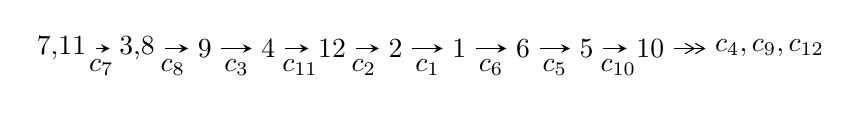
\begin{tikzpicture}[x=23pt, y=7pt]
	% node
	\node (A0) at (-1/8, 0) {7,11};
	\node (A1) at (17/16, 0) {3,8};
	\node (A2) at (17/8, 0) {9};
	\node (A3) at (25/8, 0) {4};
	\node (A4) at (33/8, 0) {12};
	\node (A5) at (41/8, 0) {2};
	\node (A6) at (49/8, 0) {1};
	\node (A7) at (57/8, 0) {6};
	\node (A8) at (65/8, 0) {5};
	\node (A9) at (73/8, 0) {10};
	\node (C1) at (1/2, -1) {$c_{7}$};
	\node (C2) at (13/8, -1) {$c_{8}$};
	\node (C3) at (21/8, -1) {$c_{3}$};
	\node (C4) at (29/8, -1) {$c_{11}$};
	\node (C5) at (37/8, -1) {$c_{2}$};
	\node (C6) at (45/8, -1) {$c_{1}$};
	\node (C7) at (53/8, -1) {$c_{6}$};
	\node (C8) at (61/8, -1) {$c_{5}$};
	\node (C9) at (69/8, -1) {$c_{10}$};
	\node (A10) at (11, 0) {$c_{4},c_{9},c_{12}$};

	% edge
	\draw[->,>=stealth]	
	(A0) edge (A1) (A1) edge (A2) (A2) edge (A3) (A3) edge (A4) (A4) edge (A5) (A5) edge (A6) (A6) edge (A7) (A7) edge (A8) (A8) edge (A9) ;
	\draw[->>,>={angle 60}]	
	(A9) edge (A10);
\end{tikzpicture} \\ 

\end{tabular} \\

\footnotetext{
The image of knot diagram is generated by the software ``\textbf{Draw programme}" developed by Andrew Bartholomew(\url{http://www.layer8.co.uk/maths/draw/index.htm\#Running-draw}), where we modified some parts for our purpose(\url{https://github.com/CATsTAILs/LinksPainter}).
}\phantom \\ \newline 
\centering \textbf{Ideals for irreducible components\footnotemark of $X_{\text{par}}$} 
 
\begin{align*}
I^u_{1}&=\langle 
6.26301\times10^{781} u^{160}+2.05461\times10^{782} u^{159}+\cdots+7.41094\times10^{783} b+8.17872\times10^{783},\\
\phantom{I^u_{1}}&\phantom{= \langle  }-3.42248\times10^{785} u^{160}-8.64272\times10^{785} u^{159}+\cdots+1.13610\times10^{787} a-1.23563\times10^{787},\\
\phantom{I^u_{1}}&\phantom{= \langle  }u^{161}+2 u^{160}+\cdots-1987 u-511\rangle \\
I^u_{2}&=\langle 
1.17622\times10^{28} u^{40}-7.67187\times10^{28} u^{39}+\cdots+9.79273\times10^{25} b-2.12717\times10^{28},\\
\phantom{I^u_{2}}&\phantom{= \langle  }1.01705\times10^{28} u^{40}-7.04668\times10^{28} u^{39}+\cdots+9.79273\times10^{25} a-3.82093\times10^{28},\;u^{41}-7 u^{40}+\cdots-11 u+1\rangle \\
I^u_{3}&=\langle 
24 a^3-33 a^2+111 b+101 a-11,\;3 a^4-6 a^3+10 a^2-11 a+13,\;u+1\rangle \\
\\
\end{align*}
\raggedright * 3 irreducible components of $\dim_{\mathbb{C}}=0$, with total 206 representations.\\
\footnotetext{All coefficients of polynomials are rational numbers. But the coefficients are sometimes approximated in decimal forms when there is not enough margin.}
\newpage
\renewcommand{\arraystretch}{1}
\centering \section*{I. $I^u_{1}= \langle 6.26\times10^{781} u^{160}+2.05\times10^{782} u^{159}+\cdots+7.41\times10^{783} b+8.18\times10^{783},\;-3.42\times10^{785} u^{160}-8.64\times10^{785} u^{159}+\cdots+1.14\times10^{787} a-1.24\times10^{787},\;u^{161}+2 u^{160}+\cdots-1987 u-511 \rangle$}
\flushleft \textbf{(i) Arc colorings}\\
\begin{tabular}{m{7pt} m{180pt} m{7pt} m{180pt} }
\flushright $a_{7}=$&$\begin{pmatrix}1\\0\end{pmatrix}$ \\
\flushright $a_{11}=$&$\begin{pmatrix}0\\u\end{pmatrix}$ \\
\flushright $a_{3}=$&$\begin{pmatrix}0.0301249 u^{160}+0.0760738 u^{159}+\cdots+110.911 u+1.08761\\-0.00845103 u^{160}-0.0277240 u^{159}+\cdots+5.96229 u-1.10360\end{pmatrix}$ \\
\flushright $a_{8}=$&$\begin{pmatrix}1\\- u^2\end{pmatrix}$ \\
\flushright $a_{9}=$&$\begin{pmatrix}-0.00881064 u^{160}-0.0336941 u^{159}+\cdots+219.424 u+43.1613\\0.00976562 u^{160}+0.0203462 u^{159}+\cdots+92.4712 u+16.6248\end{pmatrix}$ \\
\flushright $a_{4}=$&$\begin{pmatrix}0.0730709 u^{160}+0.216943 u^{159}+\cdots+146.481 u+13.8907\\0.00217044 u^{160}+0.0192015 u^{159}+\cdots-88.0122 u-12.4822\end{pmatrix}$ \\
\flushright $a_{12}=$&$\begin{pmatrix}u\\- u^3+u\end{pmatrix}$ \\
\flushright $a_{2}=$&$\begin{pmatrix}0.0216739 u^{160}+0.0483497 u^{159}+\cdots+116.873 u-0.0159891\\-0.00845103 u^{160}-0.0277240 u^{159}+\cdots+5.96229 u-1.10360\end{pmatrix}$ \\
\flushright $a_{1}=$&$\begin{pmatrix}0.0460419 u^{160}+0.109056 u^{159}+\cdots+312.046 u+70.7585\\0.00383581 u^{160}+0.0169844 u^{159}+\cdots-64.9393 u-8.15623\end{pmatrix}$ \\
\flushright $a_{6}=$&$\begin{pmatrix}-0.00323035 u^{160}-0.0113517 u^{159}+\cdots-118.318 u-22.2817\\-5.42712\times10^{-6} u^{160}+0.00842361 u^{159}+\cdots-64.3455 u-9.81544\end{pmatrix}$ \\
\flushright $a_{5}=$&$\begin{pmatrix}-0.00906781 u^{160}-0.0286508 u^{159}+\cdots-135.009 u-26.5200\\-0.00307313 u^{160}-0.00221306 u^{159}+\cdots-66.8784 u-11.1797\end{pmatrix}$ \\
\flushright $a_{10}=$&$\begin{pmatrix}-0.00399479 u^{160}+0.0136284 u^{159}+\cdots-191.412 u-46.1352\\0.00595955 u^{160}+0.0160355 u^{159}+\cdots+22.3939 u+4.62095\end{pmatrix}$\\&\end{tabular}
\flushleft \textbf{(ii) Obstruction class $= -1$}\\~\\
\flushleft \textbf{(iii) Cusp Shapes $= -0.447878 u^{160}-1.11569 u^{159}+\cdots-2252.93 u-423.424$}\\~\\
\newpage\renewcommand{\arraystretch}{1}
\flushleft \textbf{(iv) u-Polynomials at the component}\newline \\
\begin{tabular}{m{50pt}|m{274pt}}
Crossings & \hspace{64pt}u-Polynomials at each crossing \\
\hline $$\begin{aligned}c_{1}\end{aligned}$$&$\begin{aligned}
&u^{161}-9 u^{160}+\cdots-7368 u+1008
\end{aligned}$\\
\hline $$\begin{aligned}c_{2},c_{6}\end{aligned}$$&$\begin{aligned}
&u^{161}-2 u^{160}+\cdots+1477 u-211
\end{aligned}$\\
\hline $$\begin{aligned}c_{3},c_{8}\end{aligned}$$&$\begin{aligned}
&3(3 u^{161}+3 u^{160}+\cdots-1617931 u-688369)
\end{aligned}$\\
\hline $$\begin{aligned}c_{4}\end{aligned}$$&$\begin{aligned}
&3(3 u^{161}-3 u^{160}+\cdots-360 u-67)
\end{aligned}$\\
\hline $$\begin{aligned}c_{5},c_{12}\end{aligned}$$&$\begin{aligned}
&u^{161}-3 u^{160}+\cdots+72893 u+10561
\end{aligned}$\\
\hline $$\begin{aligned}c_{7},c_{11}\end{aligned}$$&$\begin{aligned}
&u^{161}+2 u^{160}+\cdots-1987 u-511
\end{aligned}$\\
\hline $$\begin{aligned}c_{9}\end{aligned}$$&$\begin{aligned}
&u^{161}-6 u^{160}+\cdots-971313 u-191967
\end{aligned}$\\
\hline $$\begin{aligned}c_{10}\end{aligned}$$&$\begin{aligned}
&3(3 u^{161}-6 u^{160}+\cdots+53653 u-3073)
\end{aligned}$\\
\hline
\end{tabular}\\~\\
\newpage\renewcommand{\arraystretch}{1}
\flushleft \textbf{(v) Riley Polynomials at the component}\newline \\
\begin{tabular}{m{50pt}|m{274pt}}
Crossings & \hspace{64pt}Riley Polynomials at each crossing \\
\hline $$\begin{aligned}c_{1}\end{aligned}$$&$\begin{aligned}
&y^{161}-19 y^{160}+\cdots-34239168 y-1016064
\end{aligned}$\\
\hline $$\begin{aligned}c_{2},c_{6}\end{aligned}$$&$\begin{aligned}
&y^{161}-96 y^{160}+\cdots+8727171 y-44521
\end{aligned}$\\
\hline $$\begin{aligned}c_{3},c_{8}\end{aligned}$$&$\begin{aligned}
&9(9 y^{161}-993 y^{160}+\cdots+6.36274\times10^{12} y-4.73852\times10^{11})
\end{aligned}$\\
\hline $$\begin{aligned}c_{4}\end{aligned}$$&$\begin{aligned}
&9(9 y^{161}+375 y^{160}+\cdots-456918 y-4489)
\end{aligned}$\\
\hline $$\begin{aligned}c_{5},c_{12}\end{aligned}$$&$\begin{aligned}
&y^{161}+125 y^{160}+\cdots-2360486615 y-111534721
\end{aligned}$\\
\hline $$\begin{aligned}c_{7},c_{11}\end{aligned}$$&$\begin{aligned}
&y^{161}-72 y^{160}+\cdots+12901911 y-261121
\end{aligned}$\\
\hline $$\begin{aligned}c_{9}\end{aligned}$$&$\begin{aligned}
&y^{161}+66 y^{160}+\cdots-2734308592791 y-36851329089
\end{aligned}$\\
\hline $$\begin{aligned}c_{10}\end{aligned}$$&$\begin{aligned}
&9(9 y^{161}+240 y^{160}+\cdots-7.15932\times10^{9} y-9443329)
\end{aligned}$\\
\hline
\end{tabular}\\~\\
\newpage\flushleft \textbf{(vi) Complex Volumes and Cusp Shapes}
$$\begin{array}{c|c|c}  
\text{Solutions to }I^u_{1}& \I (\text{vol} + \sqrt{-1}CS) & \text{Cusp shape}\\
 \hline 
\begin{aligned}
u &= -0.307620 + 0.952167 I \\
a &= \phantom{-}0.866623 - 0.790009 I \\
b &= \phantom{-}1.012620 + 0.071160 I\end{aligned}
 & -6.60700 + 2.07406 I & \phantom{-0.000000 } 0 \\ \hline\begin{aligned}
u &= -0.307620 - 0.952167 I \\
a &= \phantom{-}0.866623 + 0.790009 I \\
b &= \phantom{-}1.012620 - 0.071160 I\end{aligned}
 & -6.60700 - 2.07406 I & \phantom{-0.000000 } 0 \\ \hline\begin{aligned}
u &= -0.694056 + 0.721930 I \\
a &= -0.330278 + 0.483316 I \\
b &= \phantom{-}1.239190 - 0.345554 I\end{aligned}
 & -9.53706 - 1.18119 I & \phantom{-0.000000 } 0 \\ \hline\begin{aligned}
u &= -0.694056 - 0.721930 I \\
a &= -0.330278 - 0.483316 I \\
b &= \phantom{-}1.239190 + 0.345554 I\end{aligned}
 & -9.53706 + 1.18119 I & \phantom{-0.000000 } 0 \\ \hline\begin{aligned}
u &= \phantom{-}0.757194 + 0.665062 I \\
a &= -0.886099 - 0.367909 I \\
b &= -0.913713 + 0.411469 I\end{aligned}
 & -0.86721 + 3.70442 I & \phantom{-0.000000 } 0 \\ \hline\begin{aligned}
u &= \phantom{-}0.757194 - 0.665062 I \\
a &= -0.886099 + 0.367909 I \\
b &= -0.913713 - 0.411469 I\end{aligned}
 & -0.86721 - 3.70442 I & \phantom{-0.000000 } 0 \\ \hline\begin{aligned}
u &= \phantom{-}1.000180 + 0.136656 I \\
a &= -1.48453 - 0.76706 I \\
b &= \phantom{-}0.696245 + 0.987721 I\end{aligned}
 & \phantom{-}2.08414 - 2.27177 I & \phantom{-0.000000 } 0 \\ \hline\begin{aligned}
u &= \phantom{-}1.000180 - 0.136656 I \\
a &= -1.48453 + 0.76706 I \\
b &= \phantom{-}0.696245 - 0.987721 I\end{aligned}
 & \phantom{-}2.08414 + 2.27177 I & \phantom{-0.000000 } 0 \\ \hline\begin{aligned}
u &= -1.010580 + 0.202660 I \\
a &= \phantom{-}0.14322 + 1.42243 I \\
b &= -0.353449 - 1.049120 I\end{aligned}
 & \phantom{-}1.54662 - 3.90229 I & \phantom{-0.000000 } 0 \\ \hline\begin{aligned}
u &= -1.010580 - 0.202660 I \\
a &= \phantom{-}0.14322 - 1.42243 I \\
b &= -0.353449 + 1.049120 I\end{aligned}
 & \phantom{-}1.54662 + 3.90229 I & \phantom{-0.000000 } 0\\
 \hline 
 \end{array}$$\newpage$$\begin{array}{c|c|c}  
\text{Solutions to }I^u_{1}& \I (\text{vol} + \sqrt{-1}CS) & \text{Cusp shape}\\
 \hline 
\begin{aligned}
u &= -0.937649 + 0.480925 I \\
a &= -0.55660 + 1.64914 I \\
b &= -0.051191 - 1.321570 I\end{aligned}
 & \phantom{-}0.65918 - 4.35120 I & \phantom{-0.000000 } 0 \\ \hline\begin{aligned}
u &= -0.937649 - 0.480925 I \\
a &= -0.55660 - 1.64914 I \\
b &= -0.051191 + 1.321570 I\end{aligned}
 & \phantom{-}0.65918 + 4.35120 I & \phantom{-0.000000 } 0 \\ \hline\begin{aligned}
u &= -0.858875 + 0.384915 I \\
a &= \phantom{-}0.726945 - 0.833196 I \\
b &= -0.821170 + 0.835424 I\end{aligned}
 & -0.825469 + 0.869464 I & \phantom{-0.000000 } 0 \\ \hline\begin{aligned}
u &= -0.858875 - 0.384915 I \\
a &= \phantom{-}0.726945 + 0.833196 I \\
b &= -0.821170 - 0.835424 I\end{aligned}
 & -0.825469 - 0.869464 I & \phantom{-0.000000 } 0 \\ \hline\begin{aligned}
u &= -0.419403 + 0.975159 I \\
a &= \phantom{-}0.057520 - 0.189889 I \\
b &= \phantom{-}1.41069 - 0.39658 I\end{aligned}
 & -6.64563 + 5.26029 I & \phantom{-0.000000 } 0 \\ \hline\begin{aligned}
u &= -0.419403 - 0.975159 I \\
a &= \phantom{-}0.057520 + 0.189889 I \\
b &= \phantom{-}1.41069 + 0.39658 I\end{aligned}
 & -6.64563 - 5.26029 I & \phantom{-0.000000 } 0 \\ \hline\begin{aligned}
u &= -0.859602 + 0.324491 I \\
a &= \phantom{-}0.250764 + 1.122800 I \\
b &= -1.182960 - 0.369855 I\end{aligned}
 & -1.51059 - 1.54088 I & \phantom{-0.000000 } 0 \\ \hline\begin{aligned}
u &= -0.859602 - 0.324491 I \\
a &= \phantom{-}0.250764 - 1.122800 I \\
b &= -1.182960 + 0.369855 I\end{aligned}
 & -1.51059 + 1.54088 I & \phantom{-0.000000 } 0 \\ \hline\begin{aligned}
u &= -0.808002 + 0.437102 I \\
a &= \phantom{-}1.14632 - 1.42956 I \\
b &= -0.60913 + 1.29036 I\end{aligned}
 & \phantom{-}0.161696 + 0.583000 I & \phantom{-0.000000 } 0 \\ \hline\begin{aligned}
u &= -0.808002 - 0.437102 I \\
a &= \phantom{-}1.14632 + 1.42956 I \\
b &= -0.60913 - 1.29036 I\end{aligned}
 & \phantom{-}0.161696 - 0.583000 I & \phantom{-0.000000 } 0\\
 \hline 
 \end{array}$$\newpage$$\begin{array}{c|c|c}  
\text{Solutions to }I^u_{1}& \I (\text{vol} + \sqrt{-1}CS) & \text{Cusp shape}\\
 \hline 
\begin{aligned}
u &= \phantom{-}0.985990 + 0.448382 I \\
a &= \phantom{-}0.51871 + 1.55479 I \\
b &= -0.393892 - 1.326190 I\end{aligned}
 & \phantom{-}0.70368 + 6.58930 I & \phantom{-0.000000 } 0 \\ \hline\begin{aligned}
u &= \phantom{-}0.985990 - 0.448382 I \\
a &= \phantom{-}0.51871 - 1.55479 I \\
b &= -0.393892 + 1.326190 I\end{aligned}
 & \phantom{-}0.70368 - 6.58930 I & \phantom{-0.000000 } 0 \\ \hline\begin{aligned}
u &= -0.455529 + 0.790509 I \\
a &= \phantom{-}0.320006 + 0.168144 I \\
b &= -1.339760 + 0.406077 I\end{aligned}
 & -4.19116 + 1.49970 I & \phantom{-0.000000 } 0 \\ \hline\begin{aligned}
u &= -0.455529 - 0.790509 I \\
a &= \phantom{-}0.320006 - 0.168144 I \\
b &= -1.339760 - 0.406077 I\end{aligned}
 & -4.19116 - 1.49970 I & \phantom{-0.000000 } 0 \\ \hline\begin{aligned}
u &= \phantom{-}0.803804 + 0.418287 I \\
a &= \phantom{-}0.592060 + 0.658989 I \\
b &= \phantom{-}0.592812 - 0.098081 I\end{aligned}
 & \phantom{-}1.26994 + 0.65097 I & \phantom{-0.000000 } 0 \\ \hline\begin{aligned}
u &= \phantom{-}0.803804 - 0.418287 I \\
a &= \phantom{-}0.592060 - 0.658989 I \\
b &= \phantom{-}0.592812 + 0.098081 I\end{aligned}
 & \phantom{-}1.26994 - 0.65097 I & \phantom{-0.000000 } 0 \\ \hline\begin{aligned}
u &= \phantom{-}0.955278 + 0.547579 I \\
a &= -0.663249 - 1.208280 I \\
b &= -1.327180 + 0.459083 I\end{aligned}
 & -2.03806 + 5.71043 I & \phantom{-0.000000 } 0 \\ \hline\begin{aligned}
u &= \phantom{-}0.955278 - 0.547579 I \\
a &= -0.663249 + 1.208280 I \\
b &= -1.327180 - 0.459083 I\end{aligned}
 & -2.03806 - 5.71043 I & \phantom{-0.000000 } 0 \\ \hline\begin{aligned}
u &= -0.191812 + 0.875991 I \\
a &= -1.139400 - 0.259186 I \\
b &= -1.000060 + 0.426340 I\end{aligned}
 & -4.71556 + 7.72629 I & \phantom{-0.000000 } 0 \\ \hline\begin{aligned}
u &= -0.191812 - 0.875991 I \\
a &= -1.139400 + 0.259186 I \\
b &= -1.000060 - 0.426340 I\end{aligned}
 & -4.71556 - 7.72629 I & \phantom{-0.000000 } 0\\
 \hline 
 \end{array}$$\newpage$$\begin{array}{c|c|c}  
\text{Solutions to }I^u_{1}& \I (\text{vol} + \sqrt{-1}CS) & \text{Cusp shape}\\
 \hline 
\begin{aligned}
u &= -0.184694 + 1.096180 I \\
a &= \phantom{-}0.939637 - 0.544248 I \\
b &= \phantom{-}0.936750 + 0.091000 I\end{aligned}
 & -6.60534 + 2.09068 I & \phantom{-0.000000 } 0 \\ \hline\begin{aligned}
u &= -0.184694 - 1.096180 I \\
a &= \phantom{-}0.939637 + 0.544248 I \\
b &= \phantom{-}0.936750 - 0.091000 I\end{aligned}
 & -6.60534 - 2.09068 I & \phantom{-0.000000 } 0 \\ \hline\begin{aligned}
u &= \phantom{-}0.003922 + 1.111630 I \\
a &= -0.010112 + 0.157415 I \\
b &= \phantom{-}1.272180 + 0.011915 I\end{aligned}
 & -7.46914 + 2.60399 I & \phantom{-0.000000 } 0 \\ \hline\begin{aligned}
u &= \phantom{-}0.003922 - 1.111630 I \\
a &= -0.010112 - 0.157415 I \\
b &= \phantom{-}1.272180 - 0.011915 I\end{aligned}
 & -7.46914 - 2.60399 I & \phantom{-0.000000 } 0 \\ \hline\begin{aligned}
u &= \phantom{-}0.854194 + 0.217676 I \\
a &= -0.94349 - 1.76774 I \\
b &= -1.052330 + 0.212840 I\end{aligned}
 & -0.385901 + 0.880521 I & \phantom{-0.000000 } 0 \\ \hline\begin{aligned}
u &= \phantom{-}0.854194 - 0.217676 I \\
a &= -0.94349 + 1.76774 I \\
b &= -1.052330 - 0.212840 I\end{aligned}
 & -0.385901 - 0.880521 I & \phantom{-0.000000 } 0 \\ \hline\begin{aligned}
u &= \phantom{-}0.032139 + 1.119890 I \\
a &= -1.158780 + 0.171505 I \\
b &= -0.396381 + 0.036617 I\end{aligned}
 & -6.87436 - 0.19637 I & \phantom{-0.000000 } 0 \\ \hline\begin{aligned}
u &= \phantom{-}0.032139 - 1.119890 I \\
a &= -1.158780 - 0.171505 I \\
b &= -0.396381 - 0.036617 I\end{aligned}
 & -6.87436 + 0.19637 I & \phantom{-0.000000 } 0 \\ \hline\begin{aligned}
u &= \phantom{-}0.695042 + 0.536591 I \\
a &= -0.46289 - 1.57307 I \\
b &= -1.040120 - 0.236485 I\end{aligned}
 & -2.85536 - 1.30798 I & \phantom{-0.000000 } 0 \\ \hline\begin{aligned}
u &= \phantom{-}0.695042 - 0.536591 I \\
a &= -0.46289 + 1.57307 I \\
b &= -1.040120 + 0.236485 I\end{aligned}
 & -2.85536 + 1.30798 I & \phantom{-0.000000 } 0\\
 \hline 
 \end{array}$$\newpage$$\begin{array}{c|c|c}  
\text{Solutions to }I^u_{1}& \I (\text{vol} + \sqrt{-1}CS) & \text{Cusp shape}\\
 \hline 
\begin{aligned}
u &= \phantom{-}0.985279 + 0.538650 I \\
a &= \phantom{-}0.76199 - 1.93563 I \\
b &= -1.36833 + 0.52170 I\end{aligned}
 & -9.89158 - 2.57237 I & \phantom{-0.000000 } 0 \\ \hline\begin{aligned}
u &= \phantom{-}0.985279 - 0.538650 I \\
a &= \phantom{-}0.76199 + 1.93563 I \\
b &= -1.36833 - 0.52170 I\end{aligned}
 & -9.89158 + 2.57237 I & \phantom{-0.000000 } 0 \\ \hline\begin{aligned}
u &= -1.022010 + 0.467580 I \\
a &= \phantom{-}0.91171 + 2.08493 I \\
b &= -1.294080 - 0.239306 I\end{aligned}
 & -9.30991 - 8.55394 I & \phantom{-0.000000 } 0 \\ \hline\begin{aligned}
u &= -1.022010 - 0.467580 I \\
a &= \phantom{-}0.91171 - 2.08493 I \\
b &= -1.294080 + 0.239306 I\end{aligned}
 & -9.30991 + 8.55394 I & \phantom{-0.000000 } 0 \\ \hline\begin{aligned}
u &= \phantom{-}0.851820 + 0.169769 I \\
a &= -0.67708 + 4.78281 I \\
b &= \phantom{-}0.965814 - 0.093885 I\end{aligned}
 & -5.31714 + 0.40817 I & \phantom{-0.000000 } 0 \\ \hline\begin{aligned}
u &= \phantom{-}0.851820 - 0.169769 I \\
a &= -0.67708 - 4.78281 I \\
b &= \phantom{-}0.965814 + 0.093885 I\end{aligned}
 & -5.31714 - 0.40817 I & \phantom{-0.000000 } 0 \\ \hline\begin{aligned}
u &= -0.921455 + 0.656767 I \\
a &= -0.38602 + 1.51307 I \\
b &= -0.640684 - 0.634913 I\end{aligned}
 & -0.44077 - 4.98095 I & \phantom{-0.000000 } 0 \\ \hline\begin{aligned}
u &= -0.921455 - 0.656767 I \\
a &= -0.38602 - 1.51307 I \\
b &= -0.640684 + 0.634913 I\end{aligned}
 & -0.44077 + 4.98095 I & \phantom{-0.000000 } 0 \\ \hline\begin{aligned}
u &= -0.271216 + 0.819246 I \\
a &= -1.24613 + 0.85630 I \\
b &= \phantom{-}0.041868 - 0.347528 I\end{aligned}
 & -6.88233 - 0.33258 I & \phantom{-0.000000 } 0 \\ \hline\begin{aligned}
u &= -0.271216 - 0.819246 I \\
a &= -1.24613 - 0.85630 I \\
b &= \phantom{-}0.041868 + 0.347528 I\end{aligned}
 & -6.88233 + 0.33258 I & \phantom{-0.000000 } 0\\
 \hline 
 \end{array}$$\newpage$$\begin{array}{c|c|c}  
\text{Solutions to }I^u_{1}& \I (\text{vol} + \sqrt{-1}CS) & \text{Cusp shape}\\
 \hline 
\begin{aligned}
u &= \phantom{-}0.693972 + 0.509299 I \\
a &= \phantom{-}0.507902 - 0.115093 I \\
b &= -1.70331 - 0.29314 I\end{aligned}
 & -10.85730 + 6.84553 I & \phantom{-0.000000 } 0 \\ \hline\begin{aligned}
u &= \phantom{-}0.693972 - 0.509299 I \\
a &= \phantom{-}0.507902 + 0.115093 I \\
b &= -1.70331 + 0.29314 I\end{aligned}
 & -10.85730 - 6.84553 I & \phantom{-0.000000 } 0 \\ \hline\begin{aligned}
u &= \phantom{-}1.117250 + 0.227880 I \\
a &= \phantom{-}0.766964 + 0.706263 I \\
b &= \phantom{-}0.007454 - 0.728885 I\end{aligned}
 & \phantom{-}2.12196 + 1.12457 I & \phantom{-0.000000 } 0 \\ \hline\begin{aligned}
u &= \phantom{-}1.117250 - 0.227880 I \\
a &= \phantom{-}0.766964 - 0.706263 I \\
b &= \phantom{-}0.007454 + 0.728885 I\end{aligned}
 & \phantom{-}2.12196 - 1.12457 I & \phantom{-0.000000 } 0 \\ \hline\begin{aligned}
u &= -1.033530 + 0.481715 I \\
a &= -0.472882 + 0.393165 I \\
b &= -1.003090 - 0.207258 I\end{aligned}
 & \phantom{-}0.402697 + 0.643428 I & \phantom{-0.000000 } 0 \\ \hline\begin{aligned}
u &= -1.033530 - 0.481715 I \\
a &= -0.472882 - 0.393165 I \\
b &= -1.003090 + 0.207258 I\end{aligned}
 & \phantom{-}0.402697 - 0.643428 I & \phantom{-0.000000 } 0 \\ \hline\begin{aligned}
u &= \phantom{-}0.017597 + 0.857790 I \\
a &= -0.231783 + 0.317848 I \\
b &= -0.284232 - 0.556968 I\end{aligned}
 & -2.74068 + 3.84729 I & \phantom{-0.000000 } 0 \\ \hline\begin{aligned}
u &= \phantom{-}0.017597 - 0.857790 I \\
a &= -0.231783 - 0.317848 I \\
b &= -0.284232 + 0.556968 I\end{aligned}
 & -2.74068 - 3.84729 I & \phantom{-0.000000 } 0 \\ \hline\begin{aligned}
u &= -0.950675 + 0.647649 I \\
a &= -0.33656 - 1.86089 I \\
b &= \phantom{-}1.006750 + 0.574344 I\end{aligned}
 & -8.74792 - 4.04244 I & \phantom{-0.000000 } 0 \\ \hline\begin{aligned}
u &= -0.950675 - 0.647649 I \\
a &= -0.33656 + 1.86089 I \\
b &= \phantom{-}1.006750 - 0.574344 I\end{aligned}
 & -8.74792 + 4.04244 I & \phantom{-0.000000 } 0\\
 \hline 
 \end{array}$$\newpage$$\begin{array}{c|c|c}  
\text{Solutions to }I^u_{1}& \I (\text{vol} + \sqrt{-1}CS) & \text{Cusp shape}\\
 \hline 
\begin{aligned}
u &= -0.735215 + 0.409795 I \\
a &= -0.23133 + 1.79689 I \\
b &= \phantom{-}0.104232 - 0.269080 I\end{aligned}
 & -0.76863 - 4.77869 I & \phantom{-0.000000 } 0 \\ \hline\begin{aligned}
u &= -0.735215 - 0.409795 I \\
a &= -0.23133 - 1.79689 I \\
b &= \phantom{-}0.104232 + 0.269080 I\end{aligned}
 & -0.76863 + 4.77869 I & \phantom{-0.000000 } 0 \\ \hline\begin{aligned}
u &= -1.158840 + 0.039032 I \\
a &= \phantom{-}0.316449 - 0.934287 I \\
b &= \phantom{-}0.760558 + 0.517548 I\end{aligned}
 & -0.93293 + 5.77134 I & \phantom{-0.000000 } 0 \\ \hline\begin{aligned}
u &= -1.158840 - 0.039032 I \\
a &= \phantom{-}0.316449 + 0.934287 I \\
b &= \phantom{-}0.760558 - 0.517548 I\end{aligned}
 & -0.93293 - 5.77134 I & \phantom{-0.000000 } 0 \\ \hline\begin{aligned}
u &= -0.804022 + 0.239785 I \\
a &= \phantom{-}0.48327 + 2.11877 I \\
b &= -1.032630 - 0.793721 I\end{aligned}
 & -1.20518 - 3.26420 I & \phantom{-0.000000 } 0 \\ \hline\begin{aligned}
u &= -0.804022 - 0.239785 I \\
a &= \phantom{-}0.48327 - 2.11877 I \\
b &= -1.032630 + 0.793721 I\end{aligned}
 & -1.20518 + 3.26420 I & \phantom{-0.000000 } 0 \\ \hline\begin{aligned}
u &= \phantom{-}0.269887 + 1.141870 I \\
a &= \phantom{-}0.1198000 - 0.0223834 I \\
b &= -1.275770 - 0.373104 I\end{aligned}
 & -5.53964 - 7.31871 I & \phantom{-0.000000 } 0 \\ \hline\begin{aligned}
u &= \phantom{-}0.269887 - 1.141870 I \\
a &= \phantom{-}0.1198000 + 0.0223834 I \\
b &= -1.275770 + 0.373104 I\end{aligned}
 & -5.53964 + 7.31871 I & \phantom{-0.000000 } 0 \\ \hline\begin{aligned}
u &= \phantom{-}0.420657 + 0.703984 I \\
a &= \phantom{-}1.50506 + 1.07916 I \\
b &= -0.079209 - 0.914598 I\end{aligned}
 & -6.04723 - 8.13513 I & \phantom{-0.000000 } 0 \\ \hline\begin{aligned}
u &= \phantom{-}0.420657 - 0.703984 I \\
a &= \phantom{-}1.50506 - 1.07916 I \\
b &= -0.079209 + 0.914598 I\end{aligned}
 & -6.04723 + 8.13513 I & \phantom{-0.000000 } 0\\
 \hline 
 \end{array}$$\newpage$$\begin{array}{c|c|c}  
\text{Solutions to }I^u_{1}& \I (\text{vol} + \sqrt{-1}CS) & \text{Cusp shape}\\
 \hline 
\begin{aligned}
u &= -1.165150 + 0.193425 I \\
a &= -0.548727 + 1.055140 I \\
b &= \phantom{-}0.356427 - 0.913261 I\end{aligned}
 & \phantom{-}5.40078 - 2.71520 I & \phantom{-0.000000 } 0 \\ \hline\begin{aligned}
u &= -1.165150 - 0.193425 I \\
a &= -0.548727 - 1.055140 I \\
b &= \phantom{-}0.356427 + 0.913261 I\end{aligned}
 & \phantom{-}5.40078 + 2.71520 I & \phantom{-0.000000 } 0 \\ \hline\begin{aligned}
u &= \phantom{-}1.140350 + 0.318627 I \\
a &= \phantom{-}0.282837 - 0.522051 I \\
b &= -0.314726 - 0.123081 I\end{aligned}
 & \phantom{-}0.686846 + 0.619169 I & \phantom{-0.000000 } 0 \\ \hline\begin{aligned}
u &= \phantom{-}1.140350 - 0.318627 I \\
a &= \phantom{-}0.282837 + 0.522051 I \\
b &= -0.314726 + 0.123081 I\end{aligned}
 & \phantom{-}0.686846 - 0.619169 I & \phantom{-0.000000 } 0 \\ \hline\begin{aligned}
u &= \phantom{-}1.096020 + 0.467989 I \\
a &= \phantom{-}0.560109 + 1.252580 I \\
b &= \phantom{-}1.207030 - 0.201722 I\end{aligned}
 & -3.23869 + 2.03875 I & \phantom{-0.000000 } 0 \\ \hline\begin{aligned}
u &= \phantom{-}1.096020 - 0.467989 I \\
a &= \phantom{-}0.560109 - 1.252580 I \\
b &= \phantom{-}1.207030 + 0.201722 I\end{aligned}
 & -3.23869 - 2.03875 I & \phantom{-0.000000 } 0 \\ \hline\begin{aligned}
u &= \phantom{-}0.721328 + 0.359732 I \\
a &= \phantom{-}0.77747 + 1.67740 I \\
b &= \phantom{-}1.067260 - 0.771280 I\end{aligned}
 & \phantom{-}0.71088 + 4.08799 I & \phantom{-0.000000 } 0 \\ \hline\begin{aligned}
u &= \phantom{-}0.721328 - 0.359732 I \\
a &= \phantom{-}0.77747 - 1.67740 I \\
b &= \phantom{-}1.067260 + 0.771280 I\end{aligned}
 & \phantom{-}0.71088 - 4.08799 I & \phantom{-0.000000 } 0 \\ \hline\begin{aligned}
u &= -0.962638 + 0.706744 I \\
a &= -0.597389 + 0.508482 I \\
b &= \phantom{-}0.767042 - 1.071850 I\end{aligned}
 & -1.83931 + 0.56339 I & \phantom{-0.000000 } 0 \\ \hline\begin{aligned}
u &= -0.962638 - 0.706744 I \\
a &= -0.597389 - 0.508482 I \\
b &= \phantom{-}0.767042 + 1.071850 I\end{aligned}
 & -1.83931 - 0.56339 I & \phantom{-0.000000 } 0\\
 \hline 
 \end{array}$$\newpage$$\begin{array}{c|c|c}  
\text{Solutions to }I^u_{1}& \I (\text{vol} + \sqrt{-1}CS) & \text{Cusp shape}\\
 \hline 
\begin{aligned}
u &= \phantom{-}1.172650 + 0.226323 I \\
a &= \phantom{-}0.784130 - 1.062820 I \\
b &= -0.709586 + 0.108836 I\end{aligned}
 & \phantom{-}0.764169 + 0.726900 I & \phantom{-0.000000 } 0 \\ \hline\begin{aligned}
u &= \phantom{-}1.172650 - 0.226323 I \\
a &= \phantom{-}0.784130 + 1.062820 I \\
b &= -0.709586 - 0.108836 I\end{aligned}
 & \phantom{-}0.764169 - 0.726900 I & \phantom{-0.000000 } 0 \\ \hline\begin{aligned}
u &= \phantom{-}0.734739 + 0.326705 I \\
a &= -0.51537 - 2.07800 I \\
b &= \phantom{-}0.350819 + 1.184560 I\end{aligned}
 & -0.29875 - 3.16720 I & \phantom{-0.000000 } 0 \\ \hline\begin{aligned}
u &= \phantom{-}0.734739 - 0.326705 I \\
a &= -0.51537 + 2.07800 I \\
b &= \phantom{-}0.350819 - 1.184560 I\end{aligned}
 & -0.29875 + 3.16720 I & \phantom{-0.000000 } 0 \\ \hline\begin{aligned}
u &= -0.675750 + 0.432473 I \\
a &= -0.380087 + 0.086928 I \\
b &= -1.62283 + 0.12770 I\end{aligned}
 & -10.51280 + 4.76884 I & \phantom{-0.000000 } 0 \\ \hline\begin{aligned}
u &= -0.675750 - 0.432473 I \\
a &= -0.380087 - 0.086928 I \\
b &= -1.62283 - 0.12770 I\end{aligned}
 & -10.51280 - 4.76884 I & \phantom{-0.000000 } 0 \\ \hline\begin{aligned}
u &= -1.107660 + 0.467400 I \\
a &= \phantom{-}0.15975 - 1.49382 I \\
b &= \phantom{-}1.177430 + 0.577761 I\end{aligned}
 & \phantom{-}2.81006 - 8.16039 I & \phantom{-0.000000 } 0 \\ \hline\begin{aligned}
u &= -1.107660 - 0.467400 I \\
a &= \phantom{-}0.15975 + 1.49382 I \\
b &= \phantom{-}1.177430 - 0.577761 I\end{aligned}
 & \phantom{-}2.81006 + 8.16039 I & \phantom{-0.000000 } 0 \\ \hline\begin{aligned}
u &= -0.485771 + 0.624507 I \\
a &= \phantom{-}0.098286 + 0.452985 I \\
b &= \phantom{-}1.361420 + 0.036756 I\end{aligned}
 & -9.89815 - 1.88335 I & \phantom{-0.000000 } 0 \\ \hline\begin{aligned}
u &= -0.485771 - 0.624507 I \\
a &= \phantom{-}0.098286 - 0.452985 I \\
b &= \phantom{-}1.361420 - 0.036756 I\end{aligned}
 & -9.89815 + 1.88335 I & \phantom{-0.000000 } 0\\
 \hline 
 \end{array}$$\newpage$$\begin{array}{c|c|c}  
\text{Solutions to }I^u_{1}& \I (\text{vol} + \sqrt{-1}CS) & \text{Cusp shape}\\
 \hline 
\begin{aligned}
u &= -0.879991 + 0.835503 I \\
a &= \phantom{-}0.71539 - 1.39669 I \\
b &= \phantom{-}0.888029 + 0.924356 I\end{aligned}
 & -2.24651 - 6.45118 I & \phantom{-0.000000 } 0 \\ \hline\begin{aligned}
u &= -0.879991 - 0.835503 I \\
a &= \phantom{-}0.71539 + 1.39669 I \\
b &= \phantom{-}0.888029 - 0.924356 I\end{aligned}
 & -2.24651 + 6.45118 I & \phantom{-0.000000 } 0 \\ \hline\begin{aligned}
u &= \phantom{-}1.088000 + 0.543624 I \\
a &= \phantom{-}0.041343 + 1.136390 I \\
b &= -0.057012 - 1.033290 I\end{aligned}
 & -4.10644 + 4.81745 I & \phantom{-0.000000 } 0 \\ \hline\begin{aligned}
u &= \phantom{-}1.088000 - 0.543624 I \\
a &= \phantom{-}0.041343 - 1.136390 I \\
b &= -0.057012 + 1.033290 I\end{aligned}
 & -4.10644 - 4.81745 I & \phantom{-0.000000 } 0 \\ \hline\begin{aligned}
u &= \phantom{-}1.142840 + 0.458145 I \\
a &= -0.81265 + 1.69244 I \\
b &= \phantom{-}1.18734 - 0.86096 I\end{aligned}
 & -6.70805 + 4.94301 I & \phantom{-0.000000 } 0 \\ \hline\begin{aligned}
u &= \phantom{-}1.142840 - 0.458145 I \\
a &= -0.81265 - 1.69244 I \\
b &= \phantom{-}1.18734 + 0.86096 I\end{aligned}
 & -6.70805 - 4.94301 I & \phantom{-0.000000 } 0 \\ \hline\begin{aligned}
u &= \phantom{-}1.085870 + 0.600474 I \\
a &= -0.520902 - 1.258190 I \\
b &= \phantom{-}0.234438 + 1.302790 I\end{aligned}
 & -4.13261 + 13.19360 I & \phantom{-0.000000 } 0 \\ \hline\begin{aligned}
u &= \phantom{-}1.085870 - 0.600474 I \\
a &= -0.520902 + 1.258190 I \\
b &= \phantom{-}0.234438 - 1.302790 I\end{aligned}
 & -4.13261 - 13.19360 I & \phantom{-0.000000 } 0 \\ \hline\begin{aligned}
u &= \phantom{-}1.032770 + 0.719144 I \\
a &= \phantom{-}0.418032 + 1.133370 I \\
b &= \phantom{-}0.984478 - 0.525327 I\end{aligned}
 & \phantom{-}2.05779 + 4.30128 I & \phantom{-0.000000 } 0 \\ \hline\begin{aligned}
u &= \phantom{-}1.032770 - 0.719144 I \\
a &= \phantom{-}0.418032 - 1.133370 I \\
b &= \phantom{-}0.984478 + 0.525327 I\end{aligned}
 & \phantom{-}2.05779 - 4.30128 I & \phantom{-0.000000 } 0\\
 \hline 
 \end{array}$$\newpage$$\begin{array}{c|c|c}  
\text{Solutions to }I^u_{1}& \I (\text{vol} + \sqrt{-1}CS) & \text{Cusp shape}\\
 \hline 
\begin{aligned}
u &= -1.095300 + 0.624979 I \\
a &= -0.54811 - 1.43698 I \\
b &= \phantom{-}0.930832 + 0.131515 I\end{aligned}
 & -8.06950 - 3.11695 I & \phantom{-0.000000 } 0 \\ \hline\begin{aligned}
u &= -1.095300 - 0.624979 I \\
a &= -0.54811 + 1.43698 I \\
b &= \phantom{-}0.930832 - 0.131515 I\end{aligned}
 & -8.06950 + 3.11695 I & \phantom{-0.000000 } 0 \\ \hline\begin{aligned}
u &= -1.099820 + 0.623025 I \\
a &= \phantom{-}0.23410 + 1.70065 I \\
b &= -1.29773 - 0.76663 I\end{aligned}
 & -2.26951 - 6.82849 I & \phantom{-0.000000 } 0 \\ \hline\begin{aligned}
u &= -1.099820 - 0.623025 I \\
a &= \phantom{-}0.23410 - 1.70065 I \\
b &= -1.29773 + 0.76663 I\end{aligned}
 & -2.26951 + 6.82849 I & \phantom{-0.000000 } 0 \\ \hline\begin{aligned}
u &= \phantom{-}1.26971\phantom{ +0.000000I} \\
a &= \phantom{-}0.495882\phantom{ +0.000000I} \\
b &= \phantom{-}0.0792004\phantom{ +0.000000I}\end{aligned}
 & \phantom{-}2.35694\phantom{ +0.000000I} & \phantom{-0.000000 } 0 \\ \hline\begin{aligned}
u &= -1.094260 + 0.656736 I \\
a &= \phantom{-}0.039155 - 0.780404 I \\
b &= \phantom{-}1.329630 + 0.241308 I\end{aligned}
 & -4.54665 - 7.77977 I & \phantom{-0.000000 } 0 \\ \hline\begin{aligned}
u &= -1.094260 - 0.656736 I \\
a &= \phantom{-}0.039155 + 0.780404 I \\
b &= \phantom{-}1.329630 - 0.241308 I\end{aligned}
 & -4.54665 + 7.77977 I & \phantom{-0.000000 } 0 \\ \hline\begin{aligned}
u &= -1.114320 + 0.627334 I \\
a &= \phantom{-}0.326792 - 1.058440 I \\
b &= -0.250320 + 0.944682 I\end{aligned}
 & -4.62569 - 5.07135 I & \phantom{-0.000000 } 0 \\ \hline\begin{aligned}
u &= -1.114320 - 0.627334 I \\
a &= \phantom{-}0.326792 + 1.058440 I \\
b &= -0.250320 - 0.944682 I\end{aligned}
 & -4.62569 + 5.07135 I & \phantom{-0.000000 } 0 \\ \hline\begin{aligned}
u &= \phantom{-}1.211310 + 0.413659 I \\
a &= \phantom{-}0.075816 - 1.213030 I \\
b &= -0.728472 + 0.405990 I\end{aligned}
 & \phantom{-}0.931777 + 0.701045 I & \phantom{-0.000000 } 0\\
 \hline 
 \end{array}$$\newpage$$\begin{array}{c|c|c}  
\text{Solutions to }I^u_{1}& \I (\text{vol} + \sqrt{-1}CS) & \text{Cusp shape}\\
 \hline 
\begin{aligned}
u &= \phantom{-}1.211310 - 0.413659 I \\
a &= \phantom{-}0.075816 + 1.213030 I \\
b &= -0.728472 - 0.405990 I\end{aligned}
 & \phantom{-}0.931777 - 0.701045 I & \phantom{-0.000000 } 0 \\ \hline\begin{aligned}
u &= -0.206058 + 1.282840 I \\
a &= \phantom{-}0.0124771 + 0.1216520 I \\
b &= \phantom{-}1.154620 - 0.088449 I\end{aligned}
 & -7.42172 + 2.56249 I & \phantom{-0.000000 } 0 \\ \hline\begin{aligned}
u &= -0.206058 - 1.282840 I \\
a &= \phantom{-}0.0124771 - 0.1216520 I \\
b &= \phantom{-}1.154620 + 0.088449 I\end{aligned}
 & -7.42172 - 2.56249 I & \phantom{-0.000000 } 0 \\ \hline\begin{aligned}
u &= -1.169460 + 0.583060 I \\
a &= -0.37649 + 1.43236 I \\
b &= -1.232280 - 0.471962 I\end{aligned}
 & -1.93119 - 12.97130 I & \phantom{-0.000000 } 0 \\ \hline\begin{aligned}
u &= -1.169460 - 0.583060 I \\
a &= -0.37649 - 1.43236 I \\
b &= -1.232280 + 0.471962 I\end{aligned}
 & -1.93119 + 12.97130 I & \phantom{-0.000000 } 0 \\ \hline\begin{aligned}
u &= \phantom{-}1.246210 + 0.417941 I \\
a &= -0.346506 - 0.388457 I \\
b &= \phantom{-}0.638219 + 0.549929 I\end{aligned}
 & \phantom{-}3.13980 - 0.13080 I & \phantom{-0.000000 } 0 \\ \hline\begin{aligned}
u &= \phantom{-}1.246210 - 0.417941 I \\
a &= -0.346506 + 0.388457 I \\
b &= \phantom{-}0.638219 - 0.549929 I\end{aligned}
 & \phantom{-}3.13980 + 0.13080 I & \phantom{-0.000000 } 0 \\ \hline\begin{aligned}
u &= \phantom{-}0.527021 + 1.211110 I \\
a &= -0.0745299 - 0.0615258 I \\
b &= \phantom{-}1.287990 + 0.486449 I\end{aligned}
 & -10.0825 - 13.1010 I & \phantom{-0.000000 } 0 \\ \hline\begin{aligned}
u &= \phantom{-}0.527021 - 1.211110 I \\
a &= -0.0745299 + 0.0615258 I \\
b &= \phantom{-}1.287990 - 0.486449 I\end{aligned}
 & -10.0825 + 13.1010 I & \phantom{-0.000000 } 0 \\ \hline\begin{aligned}
u &= -1.261480 + 0.402454 I \\
a &= \phantom{-}0.548037 - 0.770393 I \\
b &= -0.221380 + 0.733993 I\end{aligned}
 & \phantom{-}1.23623 - 8.36689 I & \phantom{-0.000000 } 0\\
 \hline 
 \end{array}$$\newpage$$\begin{array}{c|c|c}  
\text{Solutions to }I^u_{1}& \I (\text{vol} + \sqrt{-1}CS) & \text{Cusp shape}\\
 \hline 
\begin{aligned}
u &= -1.261480 - 0.402454 I \\
a &= \phantom{-}0.548037 + 0.770393 I \\
b &= -0.221380 - 0.733993 I\end{aligned}
 & \phantom{-}1.23623 + 8.36689 I & \phantom{-0.000000 } 0 \\ \hline\begin{aligned}
u &= -1.163140 + 0.672582 I \\
a &= -0.18295 - 1.60363 I \\
b &= \phantom{-}1.49830 + 0.62235 I\end{aligned}
 & -4.37002 - 11.22320 I & \phantom{-0.000000 } 0 \\ \hline\begin{aligned}
u &= -1.163140 - 0.672582 I \\
a &= -0.18295 + 1.60363 I \\
b &= \phantom{-}1.49830 - 0.62235 I\end{aligned}
 & -4.37002 + 11.22320 I & \phantom{-0.000000 } 0 \\ \hline\begin{aligned}
u &= \phantom{-}1.224710 + 0.605505 I \\
a &= -0.524014 + 1.299420 I \\
b &= \phantom{-}1.34050 - 0.54211 I\end{aligned}
 & -4.02782 + 3.12105 I & \phantom{-0.000000 } 0 \\ \hline\begin{aligned}
u &= \phantom{-}1.224710 - 0.605505 I \\
a &= -0.524014 - 1.299420 I \\
b &= \phantom{-}1.34050 + 0.54211 I\end{aligned}
 & -4.02782 - 3.12105 I & \phantom{-0.000000 } 0 \\ \hline\begin{aligned}
u &= \phantom{-}1.364990 + 0.182342 I \\
a &= \phantom{-}0.323149 + 0.836958 I \\
b &= -0.819383 - 0.601543 I\end{aligned}
 & \phantom{-}0.67328 - 3.59709 I & \phantom{-0.000000 } 0 \\ \hline\begin{aligned}
u &= \phantom{-}1.364990 - 0.182342 I \\
a &= \phantom{-}0.323149 - 0.836958 I \\
b &= -0.819383 + 0.601543 I\end{aligned}
 & \phantom{-}0.67328 + 3.59709 I & \phantom{-0.000000 } 0 \\ \hline\begin{aligned}
u &= -1.229520 + 0.636195 I \\
a &= -0.32520 - 1.45121 I \\
b &= \phantom{-}1.226310 + 0.467301 I\end{aligned}
 & -4.23716 - 8.67666 I & \phantom{-0.000000 } 0 \\ \hline\begin{aligned}
u &= -1.229520 - 0.636195 I \\
a &= -0.32520 + 1.45121 I \\
b &= \phantom{-}1.226310 - 0.467301 I\end{aligned}
 & -4.23716 + 8.67666 I & \phantom{-0.000000 } 0 \\ \hline\begin{aligned}
u &= \phantom{-}1.406200 + 0.013882 I \\
a &= -0.868557 - 0.076576 I \\
b &= \phantom{-}0.911858 + 0.257334 I\end{aligned}
 & \phantom{-}0.15377 - 1.85758 I & \phantom{-0.000000 } 0\\
 \hline 
 \end{array}$$\newpage$$\begin{array}{c|c|c}  
\text{Solutions to }I^u_{1}& \I (\text{vol} + \sqrt{-1}CS) & \text{Cusp shape}\\
 \hline 
\begin{aligned}
u &= \phantom{-}1.406200 - 0.013882 I \\
a &= -0.868557 + 0.076576 I \\
b &= \phantom{-}0.911858 - 0.257334 I\end{aligned}
 & \phantom{-}0.15377 + 1.85758 I & \phantom{-0.000000 } 0 \\ \hline\begin{aligned}
u &= \phantom{-}1.25467 + 0.66516 I \\
a &= \phantom{-}0.30215 - 1.46481 I \\
b &= -1.32994 + 0.69700 I\end{aligned}
 & -2.48281 + 13.64050 I & \phantom{-0.000000 } 0 \\ \hline\begin{aligned}
u &= \phantom{-}1.25467 - 0.66516 I \\
a &= \phantom{-}0.30215 + 1.46481 I \\
b &= -1.32994 - 0.69700 I\end{aligned}
 & -2.48281 - 13.64050 I & \phantom{-0.000000 } 0 \\ \hline\begin{aligned}
u &= \phantom{-}0.411749 + 0.385093 I \\
a &= \phantom{-}0.648489 + 0.312236 I \\
b &= \phantom{-}0.357954 + 0.323299 I\end{aligned}
 & \phantom{-}1.146770 + 0.623643 I & \phantom{-}6.37992 - 1.17885 I \\ \hline\begin{aligned}
u &= \phantom{-}0.411749 - 0.385093 I \\
a &= \phantom{-}0.648489 - 0.312236 I \\
b &= \phantom{-}0.357954 - 0.323299 I\end{aligned}
 & \phantom{-}1.146770 - 0.623643 I & \phantom{-}6.37992 + 1.17885 I \\ \hline\begin{aligned}
u &= \phantom{-}0.499123 + 0.248148 I \\
a &= -1.122280 - 0.474782 I \\
b &= \phantom{-}1.70974 + 0.39088 I\end{aligned}
 & -9.09747 - 1.48318 I & -33.5204 - 1.1909 I \\ \hline\begin{aligned}
u &= \phantom{-}0.499123 - 0.248148 I \\
a &= -1.122280 + 0.474782 I \\
b &= \phantom{-}1.70974 - 0.39088 I\end{aligned}
 & -9.09747 + 1.48318 I & -33.5204 + 1.1909 I \\ \hline\begin{aligned}
u &= -0.66833 + 1.28724 I \\
a &= -0.019462 - 0.147584 I \\
b &= -1.137820 + 0.413007 I\end{aligned}
 & -9.73951 + 3.15623 I & \phantom{-0.000000 } 0 \\ \hline\begin{aligned}
u &= -0.66833 - 1.28724 I \\
a &= -0.019462 + 0.147584 I \\
b &= -1.137820 - 0.413007 I\end{aligned}
 & -9.73951 - 3.15623 I & \phantom{-0.000000 } 0 \\ \hline\begin{aligned}
u &= \phantom{-}1.23548 + 0.77270 I \\
a &= -0.06823 + 1.49782 I \\
b &= \phantom{-}1.36553 - 0.67981 I\end{aligned}
 & -7.7590 + 20.1115 I & \phantom{-0.000000 } 0\\
 \hline 
 \end{array}$$\newpage$$\begin{array}{c|c|c}  
\text{Solutions to }I^u_{1}& \I (\text{vol} + \sqrt{-1}CS) & \text{Cusp shape}\\
 \hline 
\begin{aligned}
u &= \phantom{-}1.23548 - 0.77270 I \\
a &= -0.06823 - 1.49782 I \\
b &= \phantom{-}1.36553 + 0.67981 I\end{aligned}
 & -7.7590 - 20.1115 I & \phantom{-0.000000 } 0 \\ \hline\begin{aligned}
u &= \phantom{-}0.482444 + 0.214250 I \\
a &= -0.91575 - 3.66564 I \\
b &= \phantom{-}0.777694 + 0.364075 I\end{aligned}
 & -6.46494 - 0.70369 I & -0.42319 + 1.37241 I \\ \hline\begin{aligned}
u &= \phantom{-}0.482444 - 0.214250 I \\
a &= -0.91575 + 3.66564 I \\
b &= \phantom{-}0.777694 - 0.364075 I\end{aligned}
 & -6.46494 + 0.70369 I & -0.42319 - 1.37241 I \\ \hline\begin{aligned}
u &= -0.037171 + 0.513665 I \\
a &= \phantom{-}1.45345 - 0.15371 I \\
b &= \phantom{-}0.824495 - 0.488952 I\end{aligned}
 & \phantom{-}0.08451 + 4.25610 I & \phantom{-}2.06157 - 6.69602 I \\ \hline\begin{aligned}
u &= -0.037171 - 0.513665 I \\
a &= \phantom{-}1.45345 + 0.15371 I \\
b &= \phantom{-}0.824495 + 0.488952 I\end{aligned}
 & \phantom{-}0.08451 - 4.25610 I & \phantom{-}2.06157 + 6.69602 I \\ \hline\begin{aligned}
u &= \phantom{-}0.69791 + 1.31654 I \\
a &= \phantom{-}0.1021750 - 0.0356810 I \\
b &= -1.173860 - 0.349159 I\end{aligned}
 & -9.80408 - 2.91263 I & \phantom{-0.000000 } 0 \\ \hline\begin{aligned}
u &= \phantom{-}0.69791 - 1.31654 I \\
a &= \phantom{-}0.1021750 + 0.0356810 I \\
b &= -1.173860 + 0.349159 I\end{aligned}
 & -9.80408 + 2.91263 I & \phantom{-0.000000 } 0 \\ \hline\begin{aligned}
u &= \phantom{-}1.22964 + 0.84982 I \\
a &= \phantom{-}0.053369 - 1.204230 I \\
b &= -1.30517 + 0.57043 I\end{aligned}
 & -7.88026 + 10.53010 I & \phantom{-0.000000 } 0 \\ \hline\begin{aligned}
u &= \phantom{-}1.22964 - 0.84982 I \\
a &= \phantom{-}0.053369 + 1.204230 I \\
b &= -1.30517 - 0.57043 I\end{aligned}
 & -7.88026 - 10.53010 I & \phantom{-0.000000 } 0 \\ \hline\begin{aligned}
u &= -1.25141 + 0.82324 I \\
a &= -0.021538 + 1.378970 I \\
b &= -1.233440 - 0.584666 I\end{aligned}
 & -7.65179 - 10.64380 I & \phantom{-0.000000 } 0\\
 \hline 
 \end{array}$$\newpage$$\begin{array}{c|c|c}  
\text{Solutions to }I^u_{1}& \I (\text{vol} + \sqrt{-1}CS) & \text{Cusp shape}\\
 \hline 
\begin{aligned}
u &= -1.25141 - 0.82324 I \\
a &= -0.021538 - 1.378970 I \\
b &= -1.233440 + 0.584666 I\end{aligned}
 & -7.65179 + 10.64380 I & \phantom{-0.000000 } 0 \\ \hline\begin{aligned}
u &= \phantom{-}0.013340 + 0.475861 I \\
a &= \phantom{-}0.826953 + 0.797491 I \\
b &= -0.314578 + 0.562221 I\end{aligned}
 & -1.12862 + 1.55624 I & \phantom{-}0.14713 - 4.64540 I \\ \hline\begin{aligned}
u &= \phantom{-}0.013340 - 0.475861 I \\
a &= \phantom{-}0.826953 - 0.797491 I \\
b &= -0.314578 - 0.562221 I\end{aligned}
 & -1.12862 - 1.55624 I & \phantom{-}0.14713 + 4.64540 I \\ \hline\begin{aligned}
u &= -0.300972 + 0.276834 I \\
a &= \phantom{-}0.957991 - 0.373426 I \\
b &= -0.634501 + 0.414017 I\end{aligned}
 & -1.22189 + 0.97193 I & -3.13839 - 0.91119 I \\ \hline\begin{aligned}
u &= -0.300972 - 0.276834 I \\
a &= \phantom{-}0.957991 + 0.373426 I \\
b &= -0.634501 - 0.414017 I\end{aligned}
 & -1.22189 - 0.97193 I & -3.13839 + 0.91119 I \\ \hline\begin{aligned}
u &= -1.62034 + 0.17971 I \\
a &= -0.694876 - 0.382724 I \\
b &= \phantom{-}0.904747 + 0.208992 I\end{aligned}
 & -0.99352 - 8.67527 I & \phantom{-0.000000 } 0 \\ \hline\begin{aligned}
u &= -1.62034 - 0.17971 I \\
a &= -0.694876 + 0.382724 I \\
b &= \phantom{-}0.904747 - 0.208992 I\end{aligned}
 & -0.99352 + 8.67527 I & \phantom{-0.000000 } 0 \\ \hline\begin{aligned}
u &= -1.65831 + 0.24819 I \\
a &= \phantom{-}0.730006 + 0.153017 I \\
b &= -0.907619 + 0.066140 I\end{aligned}
 & \phantom{-}1.07814 + 1.74223 I & \phantom{-0.000000 } 0 \\ \hline\begin{aligned}
u &= -1.65831 - 0.24819 I \\
a &= \phantom{-}0.730006 - 0.153017 I \\
b &= -0.907619 - 0.066140 I\end{aligned}
 & \phantom{-}1.07814 - 1.74223 I & \phantom{-0.000000 } 0 \\ \hline\begin{aligned}
u &= -0.226753 + 0.106637 I \\
a &= -0.28469 - 10.30590 I \\
b &= -0.473559 - 0.221475 I\end{aligned}
 & -5.59662 - 7.70854 I & -8.24793 - 2.14980 I\\
 \hline 
 \end{array}$$\newpage$$\begin{array}{c|c|c}  
\text{Solutions to }I^u_{1}& \I (\text{vol} + \sqrt{-1}CS) & \text{Cusp shape}\\
 \hline 
\begin{aligned}
u &= -0.226753 - 0.106637 I \\
a &= -0.28469 + 10.30590 I \\
b &= -0.473559 + 0.221475 I\end{aligned}
 & -5.59662 + 7.70854 I & -8.24793 + 2.14980 I\\
 \hline 
 \end{array}$$\newpage\newpage\renewcommand{\arraystretch}{1}
\centering \section*{II. $I^u_{2}= \langle 1.18\times10^{28} u^{40}-7.67\times10^{28} u^{39}+\cdots+9.79\times10^{25} b-2.13\times10^{28},\;1.02\times10^{28} u^{40}-7.05\times10^{28} u^{39}+\cdots+9.79\times10^{25} a-3.82\times10^{28},\;u^{41}-7 u^{40}+\cdots-11 u+1 \rangle$}
\flushleft \textbf{(i) Arc colorings}\\
\begin{tabular}{m{7pt} m{180pt} m{7pt} m{180pt} }
\flushright $a_{7}=$&$\begin{pmatrix}1\\0\end{pmatrix}$ \\
\flushright $a_{11}=$&$\begin{pmatrix}0\\u\end{pmatrix}$ \\
\flushright $a_{3}=$&$\begin{pmatrix}-103.857 u^{40}+719.583 u^{39}+\cdots-3148.45 u+390.180\\-120.112 u^{40}+783.425 u^{39}+\cdots-2058.58 u+217.220\end{pmatrix}$ \\
\flushright $a_{8}=$&$\begin{pmatrix}1\\- u^2\end{pmatrix}$ \\
\flushright $a_{9}=$&$\begin{pmatrix}124.264 u^{40}-817.539 u^{39}+\cdots+3063.75 u-395.819\\-55.1185 u^{40}+353.795 u^{39}+\cdots-673.835 u+63.0433\end{pmatrix}$ \\
\flushright $a_{4}=$&$\begin{pmatrix}307.135 u^{40}-1996.42 u^{39}+\cdots+5623.44 u-646.147\\195.331 u^{40}-1283.74 u^{39}+\cdots+3749.84 u-420.564\end{pmatrix}$ \\
\flushright $a_{12}=$&$\begin{pmatrix}u\\- u^3+u\end{pmatrix}$ \\
\flushright $a_{2}=$&$\begin{pmatrix}-223.969 u^{40}+1503.01 u^{39}+\cdots-5207.03 u+607.400\\-120.112 u^{40}+783.425 u^{39}+\cdots-2058.58 u+217.220\end{pmatrix}$ \\
\flushright $a_{1}=$&$\begin{pmatrix}-71.0994 u^{40}+446.847 u^{39}+\cdots-691.806 u+42.5459\\112.241 u^{40}-787.184 u^{39}+\cdots+3603.51 u-452.969\end{pmatrix}$ \\
\flushright $a_{6}=$&$\begin{pmatrix}-215.948 u^{40}+1447.88 u^{39}+\cdots-5228.86 u+629.808\\63.8011 u^{40}-427.927 u^{39}+\cdots+1300.88 u-145.479\end{pmatrix}$ \\
\flushright $a_{5}=$&$\begin{pmatrix}-227.513 u^{40}+1540.45 u^{39}+\cdots-5878.18 u+713.136\\36.9235 u^{40}-240.586 u^{39}+\cdots+512.290 u-50.5412\end{pmatrix}$ \\
\flushright $a_{10}=$&$\begin{pmatrix}-64.0733 u^{40}+471.524 u^{39}+\cdots-3124.37 u+446.988\\-164.675 u^{40}+1097.03 u^{39}+\cdots-3882.64 u+475.560\end{pmatrix}$\\&\end{tabular}
\flushleft \textbf{(ii) Obstruction class $= 1$}\\~\\
\flushleft \textbf{(iii) Cusp Shapes $= -\frac{69151959893570817174266446784}{97927278772762685526176667} u^{40}+\frac{461052684880726699730660001043}{97927278772762685526176667} u^{39}+\cdots-\frac{1296998207775107934587459370884}{97927278772762685526176667} u+\frac{132975992063944991565103362257}{97927278772762685526176667}$}\\~\\
\newpage\renewcommand{\arraystretch}{1}
\flushleft \textbf{(iv) u-Polynomials at the component}\newline \\
\begin{tabular}{m{50pt}|m{274pt}}
Crossings & \hspace{64pt}u-Polynomials at each crossing \\
\hline $$\begin{aligned}c_{1}\end{aligned}$$&$\begin{aligned}
&u^{41}-8 u^{40}+\cdots-555 u+37
\end{aligned}$\\
\hline $$\begin{aligned}c_{2}\end{aligned}$$&$\begin{aligned}
&u^{41}+u^{40}+\cdots+3 u-1
\end{aligned}$\\
\hline $$\begin{aligned}c_{3}\end{aligned}$$&$\begin{aligned}
&u^{41}-9 u^{39}+\cdots+9 u^2+1
\end{aligned}$\\
\hline $$\begin{aligned}c_{4}\end{aligned}$$&$\begin{aligned}
&u^{41}+15 u^{39}+\cdots- u+1
\end{aligned}$\\
\hline $$\begin{aligned}c_{5}\end{aligned}$$&$\begin{aligned}
&u^{41}+2 u^{40}+\cdots-15 u-1
\end{aligned}$\\
\hline $$\begin{aligned}c_{6}\end{aligned}$$&$\begin{aligned}
&u^{41}- u^{40}+\cdots+3 u+1
\end{aligned}$\\
\hline $$\begin{aligned}c_{7}\end{aligned}$$&$\begin{aligned}
&u^{41}-7 u^{40}+\cdots-11 u+1
\end{aligned}$\\
\hline $$\begin{aligned}c_{8}\end{aligned}$$&$\begin{aligned}
&u^{41}-9 u^{39}+\cdots-9 u^2-1
\end{aligned}$\\
\hline $$\begin{aligned}c_{9}\end{aligned}$$&$\begin{aligned}
&u^{41}+14 u^{39}+\cdots+2 u+1
\end{aligned}$\\
\hline $$\begin{aligned}c_{10}\end{aligned}$$&$\begin{aligned}
&u^{41}+10 u^{39}+\cdots+7 u-1
\end{aligned}$\\
\hline $$\begin{aligned}c_{11}\end{aligned}$$&$\begin{aligned}
&u^{41}+7 u^{40}+\cdots-11 u-1
\end{aligned}$\\
\hline $$\begin{aligned}c_{12}\end{aligned}$$&$\begin{aligned}
&u^{41}-2 u^{40}+\cdots-15 u+1
\end{aligned}$\\
\hline
\end{tabular}\\~\\
\newpage\renewcommand{\arraystretch}{1}
\flushleft \textbf{(v) Riley Polynomials at the component}\newline \\
\begin{tabular}{m{50pt}|m{274pt}}
Crossings & \hspace{64pt}Riley Polynomials at each crossing \\
\hline $$\begin{aligned}c_{1}\end{aligned}$$&$\begin{aligned}
&y^{41}-4 y^{40}+\cdots-2701 y-1369
\end{aligned}$\\
\hline $$\begin{aligned}c_{2},c_{6}\end{aligned}$$&$\begin{aligned}
&y^{41}-27 y^{40}+\cdots+35 y-1
\end{aligned}$\\
\hline $$\begin{aligned}c_{3},c_{8}\end{aligned}$$&$\begin{aligned}
&y^{41}-18 y^{40}+\cdots-18 y-1
\end{aligned}$\\
\hline $$\begin{aligned}c_{4}\end{aligned}$$&$\begin{aligned}
&y^{41}+30 y^{40}+\cdots- y-1
\end{aligned}$\\
\hline $$\begin{aligned}c_{5},c_{12}\end{aligned}$$&$\begin{aligned}
&y^{41}+38 y^{40}+\cdots-27 y-1
\end{aligned}$\\
\hline $$\begin{aligned}c_{7},c_{11}\end{aligned}$$&$\begin{aligned}
&y^{41}-17 y^{40}+\cdots+33 y-1
\end{aligned}$\\
\hline $$\begin{aligned}c_{9}\end{aligned}$$&$\begin{aligned}
&y^{41}+28 y^{40}+\cdots+12 y-1
\end{aligned}$\\
\hline $$\begin{aligned}c_{10}\end{aligned}$$&$\begin{aligned}
&y^{41}+20 y^{40}+\cdots+61 y-1
\end{aligned}$\\
\hline
\end{tabular}\\~\\
\newpage\flushleft \textbf{(vi) Complex Volumes and Cusp Shapes}
$$\begin{array}{c|c|c}  
\text{Solutions to }I^u_{2}& \I (\text{vol} + \sqrt{-1}CS) & \text{Cusp shape}\\
 \hline 
\begin{aligned}
u &= -0.927142 + 0.347305 I \\
a &= -0.458871 + 1.255540 I \\
b &= -1.057560 - 0.222374 I\end{aligned}
 & -0.209317 - 1.191770 I & \phantom{-}3.70255 + 3.16958 I \\ \hline\begin{aligned}
u &= -0.927142 - 0.347305 I \\
a &= -0.458871 - 1.255540 I \\
b &= -1.057560 + 0.222374 I\end{aligned}
 & -0.209317 + 1.191770 I & \phantom{-}3.70255 - 3.16958 I \\ \hline\begin{aligned}
u &= -0.779419 + 0.650200 I \\
a &= \phantom{-}0.830867 - 0.924238 I \\
b &= \phantom{-}1.082080 + 0.668899 I\end{aligned}
 & -0.40581 - 4.85911 I & \phantom{-}2.00000 + 7.72188 I \\ \hline\begin{aligned}
u &= -0.779419 - 0.650200 I \\
a &= \phantom{-}0.830867 + 0.924238 I \\
b &= \phantom{-}1.082080 - 0.668899 I\end{aligned}
 & -0.40581 + 4.85911 I & \phantom{-}2.00000 - 7.72188 I \\ \hline\begin{aligned}
u &= \phantom{-}0.169274 + 0.961950 I \\
a &= -0.379003 - 0.109241 I \\
b &= \phantom{-}1.186620 + 0.201083 I\end{aligned}
 & -9.46272 - 0.62426 I & -5.91667 + 0.44319 I \\ \hline\begin{aligned}
u &= \phantom{-}0.169274 - 0.961950 I \\
a &= -0.379003 + 0.109241 I \\
b &= \phantom{-}1.186620 - 0.201083 I\end{aligned}
 & -9.46272 + 0.62426 I & -5.91667 - 0.44319 I \\ \hline\begin{aligned}
u &= \phantom{-}0.852470 + 0.470972 I \\
a &= -1.006690 - 0.985928 I \\
b &= \phantom{-}0.80738 + 1.23399 I\end{aligned}
 & \phantom{-}0.20579 - 1.47899 I & \phantom{-}4.23119 + 4.48438 I \\ \hline\begin{aligned}
u &= \phantom{-}0.852470 - 0.470972 I \\
a &= -1.006690 + 0.985928 I \\
b &= \phantom{-}0.80738 - 1.23399 I\end{aligned}
 & \phantom{-}0.20579 + 1.47899 I & \phantom{-}4.23119 - 4.48438 I \\ \hline\begin{aligned}
u &= \phantom{-}0.874084 + 0.404182 I \\
a &= \phantom{-}0.29626 + 1.99805 I \\
b &= \phantom{-}0.104278 - 1.050880 I\end{aligned}
 & \phantom{-}0.12542 + 5.23179 I & \phantom{-}2.84870 - 9.19616 I \\ \hline\begin{aligned}
u &= \phantom{-}0.874084 - 0.404182 I \\
a &= \phantom{-}0.29626 - 1.99805 I \\
b &= \phantom{-}0.104278 + 1.050880 I\end{aligned}
 & \phantom{-}0.12542 - 5.23179 I & \phantom{-}2.84870 + 9.19616 I\\
 \hline 
 \end{array}$$\newpage$$\begin{array}{c|c|c}  
\text{Solutions to }I^u_{2}& \I (\text{vol} + \sqrt{-1}CS) & \text{Cusp shape}\\
 \hline 
\begin{aligned}
u &= -0.134326 + 0.938630 I \\
a &= \phantom{-}1.92681 - 0.22109 I \\
b &= \phantom{-}0.735171 - 0.074399 I\end{aligned}
 & -7.55315 + 0.49721 I & -12.44075 - 0.83713 I \\ \hline\begin{aligned}
u &= -0.134326 - 0.938630 I \\
a &= \phantom{-}1.92681 + 0.22109 I \\
b &= \phantom{-}0.735171 + 0.074399 I\end{aligned}
 & -7.55315 - 0.49721 I & -12.44075 + 0.83713 I \\ \hline\begin{aligned}
u &= \phantom{-}0.847382 + 0.673086 I \\
a &= \phantom{-}0.59982 + 1.67848 I \\
b &= \phantom{-}0.798239 - 0.790803 I\end{aligned}
 & -0.04074 + 5.69554 I & \phantom{-0.000000 } 0. - 10.22141 I \\ \hline\begin{aligned}
u &= \phantom{-}0.847382 - 0.673086 I \\
a &= \phantom{-}0.59982 - 1.67848 I \\
b &= \phantom{-}0.798239 + 0.790803 I\end{aligned}
 & -0.04074 - 5.69554 I & \phantom{-0.000000 -}0. + 10.22141 I \\ \hline\begin{aligned}
u &= -0.814515 + 0.148698 I \\
a &= \phantom{-}0.01989 - 4.77317 I \\
b &= \phantom{-}0.983453 + 0.090171 I\end{aligned}
 & -5.36930 - 0.36776 I & -26.9936 - 46.1947 I \\ \hline\begin{aligned}
u &= -0.814515 - 0.148698 I \\
a &= \phantom{-}0.01989 + 4.77317 I \\
b &= \phantom{-}0.983453 - 0.090171 I\end{aligned}
 & -5.36930 + 0.36776 I & -26.9936 + 46.1947 I \\ \hline\begin{aligned}
u &= -0.767792 + 0.210103 I \\
a &= \phantom{-}0.25462 + 2.21185 I \\
b &= -1.055760 - 0.709790 I\end{aligned}
 & -1.14623 - 2.95576 I & \phantom{-}1.49798 - 5.01948 I \\ \hline\begin{aligned}
u &= -0.767792 - 0.210103 I \\
a &= \phantom{-}0.25462 - 2.21185 I \\
b &= -1.055760 + 0.709790 I\end{aligned}
 & -1.14623 + 2.95576 I & \phantom{-}1.49798 + 5.01948 I \\ \hline\begin{aligned}
u &= -1.206980 + 0.004858 I \\
a &= \phantom{-}0.522791 - 0.594761 I \\
b &= -0.681406 + 0.517358 I\end{aligned}
 & \phantom{-}1.05481 + 1.82958 I & \phantom{-0.000000 } 0 \\ \hline\begin{aligned}
u &= -1.206980 - 0.004858 I \\
a &= \phantom{-}0.522791 + 0.594761 I \\
b &= -0.681406 - 0.517358 I\end{aligned}
 & \phantom{-}1.05481 - 1.82958 I & \phantom{-0.000000 } 0\\
 \hline 
 \end{array}$$\newpage$$\begin{array}{c|c|c}  
\text{Solutions to }I^u_{2}& \I (\text{vol} + \sqrt{-1}CS) & \text{Cusp shape}\\
 \hline 
\begin{aligned}
u &= \phantom{-}1.130650 + 0.476710 I \\
a &= -0.74768 + 1.67148 I \\
b &= \phantom{-}1.077280 - 0.799534 I\end{aligned}
 & -6.46333 + 5.00874 I & \phantom{-0.000000 } 0 \\ \hline\begin{aligned}
u &= \phantom{-}1.130650 - 0.476710 I \\
a &= -0.74768 - 1.67148 I \\
b &= \phantom{-}1.077280 + 0.799534 I\end{aligned}
 & -6.46333 - 5.00874 I & \phantom{-0.000000 } 0 \\ \hline\begin{aligned}
u &= -1.163120 + 0.457722 I \\
a &= -0.745162 + 0.080722 I \\
b &= \phantom{-}0.646488 - 0.575713 I\end{aligned}
 & \phantom{-}1.073130 + 0.108725 I & \phantom{-0.000000 } 0 \\ \hline\begin{aligned}
u &= -1.163120 - 0.457722 I \\
a &= -0.745162 - 0.080722 I \\
b &= \phantom{-}0.646488 + 0.575713 I\end{aligned}
 & \phantom{-}1.073130 - 0.108725 I & \phantom{-0.000000 } 0 \\ \hline\begin{aligned}
u &= \phantom{-}0.50894 + 1.32024 I \\
a &= -0.0545155 + 0.0076336 I \\
b &= -1.180730 - 0.282349 I\end{aligned}
 & -7.90500 - 3.73304 I & \phantom{-0.000000 } 0 \\ \hline\begin{aligned}
u &= \phantom{-}0.50894 - 1.32024 I \\
a &= -0.0545155 - 0.0076336 I \\
b &= -1.180730 + 0.282349 I\end{aligned}
 & -7.90500 + 3.73304 I & \phantom{-0.000000 } 0 \\ \hline\begin{aligned}
u &= \phantom{-}0.13872 + 1.40852 I \\
a &= -0.671598 - 0.214370 I \\
b &= -0.704102 + 0.153201 I\end{aligned}
 & -5.88626 - 1.89602 I & \phantom{-0.000000 } 0 \\ \hline\begin{aligned}
u &= \phantom{-}0.13872 - 1.40852 I \\
a &= -0.671598 + 0.214370 I \\
b &= -0.704102 - 0.153201 I\end{aligned}
 & -5.88626 + 1.89602 I & \phantom{-0.000000 } 0 \\ \hline\begin{aligned}
u &= \phantom{-}1.23516 + 0.69600 I \\
a &= \phantom{-}0.194284 - 1.366840 I \\
b &= -1.38116 + 0.49611 I\end{aligned}
 & -5.16982 + 10.63520 I & \phantom{-0.000000 } 0 \\ \hline\begin{aligned}
u &= \phantom{-}1.23516 - 0.69600 I \\
a &= \phantom{-}0.194284 + 1.366840 I \\
b &= -1.38116 - 0.49611 I\end{aligned}
 & -5.16982 - 10.63520 I & \phantom{-0.000000 } 0\\
 \hline 
 \end{array}$$\newpage$$\begin{array}{c|c|c}  
\text{Solutions to }I^u_{2}& \I (\text{vol} + \sqrt{-1}CS) & \text{Cusp shape}\\
 \hline 
\begin{aligned}
u &= \phantom{-}0.541613 + 0.208824 I \\
a &= -0.746318 - 0.695676 I \\
b &= \phantom{-}1.67442 + 0.36291 I\end{aligned}
 & -8.94999 - 1.49636 I & \phantom{-}20.7031 + 3.0348 I \\ \hline\begin{aligned}
u &= \phantom{-}0.541613 - 0.208824 I \\
a &= -0.746318 + 0.695676 I \\
b &= \phantom{-}1.67442 - 0.36291 I\end{aligned}
 & -8.94999 + 1.49636 I & \phantom{-}20.7031 - 3.0348 I \\ \hline\begin{aligned}
u &= \phantom{-}0.505972 + 0.281568 I \\
a &= -0.09598 - 5.32389 I \\
b &= -0.507756 + 0.380061 I\end{aligned}
 & -5.43434 + 8.00305 I & \phantom{-}3.2067 - 18.2543 I \\ \hline\begin{aligned}
u &= \phantom{-}0.505972 - 0.281568 I \\
a &= -0.09598 + 5.32389 I \\
b &= -0.507756 - 0.380061 I\end{aligned}
 & -5.43434 - 8.00305 I & \phantom{-}3.2067 + 18.2543 I \\ \hline\begin{aligned}
u &= \phantom{-}1.42007 + 0.26318 I \\
a &= \phantom{-}0.257366 - 0.114072 I \\
b &= \phantom{-}0.388206 + 0.250021 I\end{aligned}
 & \phantom{-}2.23063 - 1.66443 I & \phantom{-0.000000 } 0 \\ \hline\begin{aligned}
u &= \phantom{-}1.42007 - 0.26318 I \\
a &= \phantom{-}0.257366 + 0.114072 I \\
b &= \phantom{-}0.388206 - 0.250021 I\end{aligned}
 & \phantom{-}2.23063 + 1.66443 I & \phantom{-0.000000 } 0 \\ \hline\begin{aligned}
u &= -1.44664\phantom{ +0.000000I} \\
a &= \phantom{-}0.968478\phantom{ +0.000000I} \\
b &= -0.842248\phantom{ +0.000000I}\end{aligned}
 & \phantom{-}1.38645\phantom{ +0.000000I} & \phantom{-0.000000 } 0 \\ \hline\begin{aligned}
u &= \phantom{-}1.43864 + 0.27829 I \\
a &= -0.086081 + 0.267918 I \\
b &= -0.395833 - 0.011531 I\end{aligned}
 & -0.24255 + 7.82530 I & \phantom{-0.000000 } 0 \\ \hline\begin{aligned}
u &= \phantom{-}1.43864 - 0.27829 I \\
a &= -0.086081 - 0.267918 I \\
b &= -0.395833 + 0.011531 I\end{aligned}
 & -0.24255 - 7.82530 I & \phantom{-0.000000 } 0 \\ \hline\begin{aligned}
u &= \phantom{-}0.353644 + 0.050253 I \\
a &= -0.39505 - 2.54918 I \\
b &= -1.59820 + 0.06316 I\end{aligned}
 & -10.23170 - 5.70633 I & -1.45537 + 6.02958 I\\
 \hline 
 \end{array}$$\newpage$$\begin{array}{c|c|c}  
\text{Solutions to }I^u_{2}& \I (\text{vol} + \sqrt{-1}CS) & \text{Cusp shape}\\
 \hline 
\begin{aligned}
u &= \phantom{-}0.353644 - 0.050253 I \\
a &= -0.39505 + 2.54918 I \\
b &= -1.59820 - 0.06316 I\end{aligned}
 & -10.23170 + 5.70633 I & -1.45537 - 6.02958 I\\
 \hline 
 \end{array}$$\newpage\newpage\renewcommand{\arraystretch}{1}
\centering \section*{III. $I^u_{3}= \langle 24 a^3-33 a^2+111 b+101 a-11,\;3 a^4-6 a^3+10 a^2-11 a+13,\;u+1 \rangle$}
\flushleft \textbf{(i) Arc colorings}\\
\begin{tabular}{m{7pt} m{180pt} m{7pt} m{180pt} }
\flushright $a_{7}=$&$\begin{pmatrix}1\\0\end{pmatrix}$ \\
\flushright $a_{11}=$&$\begin{pmatrix}0\\-1\end{pmatrix}$ \\
\flushright $a_{3}=$&$\begin{pmatrix}a\\-0.216216 a^{3}+0.297297 a^{2}-0.909910 a+0.0990991\end{pmatrix}$ \\
\flushright $a_{8}=$&$\begin{pmatrix}1\\-1\end{pmatrix}$ \\
\flushright $a_{9}=$&$\begin{pmatrix}-0.135135 a^{3}+0.810811 a^{2}-0.693694 a+1.93694\\0.0810811 a^{3}-0.486486 a^{2}+0.216216 a-1.16216\end{pmatrix}$ \\
\flushright $a_{4}=$&$\begin{pmatrix}\frac{1}{3} a-\frac{1}{3}\\-0.243243 a^{3}+0.459459 a^{2}-0.648649 a+0.486486\end{pmatrix}$ \\
\flushright $a_{12}=$&$\begin{pmatrix}-1\\0\end{pmatrix}$ \\
\flushright $a_{2}=$&$\begin{pmatrix}-0.216216 a^{3}+0.297297 a^{2}+0.0900901 a+0.0990991\\-0.216216 a^{3}+0.297297 a^{2}-0.909910 a+0.0990991\end{pmatrix}$ \\
\flushright $a_{1}=$&$\begin{pmatrix}-0.216216 a^{3}+0.297297 a^{2}+0.0900901 a+0.0990991\\-0.216216 a^{3}+0.297297 a^{2}-0.909910 a+0.0990991\end{pmatrix}$ \\
\flushright $a_{6}=$&$\begin{pmatrix}-0.0810811 a^{3}+0.486486 a^{2}-0.216216 a+1.16216\\-0.216216 a^{3}+0.297297 a^{2}-0.909910 a+1.09910\end{pmatrix}$ \\
\flushright $a_{5}=$&$\begin{pmatrix}0.135135 a^{3}+0.189189 a^{2}+0.693694 a+0.0630631\\-0.216216 a^{3}+0.297297 a^{2}-0.909910 a+1.09910\end{pmatrix}$ \\
\flushright $a_{10}=$&$\begin{pmatrix}0.0810811 a^{3}+0.513514 a^{2}+0.216216 a+0.837838\\-0.432432 a^{3}+0.594595 a^{2}-0.819820 a+0.198198\end{pmatrix}$\\&\end{tabular}
\flushleft \textbf{(ii) Obstruction class $= 1$}\\~\\
\flushleft \textbf{(iii) Cusp Shapes $= \frac{57}{37} a^3-\frac{397}{111} a^2+\frac{493}{111} a-\frac{40}{37}$}\\~\\
\newpage\renewcommand{\arraystretch}{1}
\flushleft \textbf{(iv) u-Polynomials at the component}\newline \\
\begin{tabular}{m{50pt}|m{274pt}}
Crossings & \hspace{64pt}u-Polynomials at each crossing \\
\hline $$\begin{aligned}c_{1}\end{aligned}$$&$\begin{aligned}
&u^4
\end{aligned}$\\
\hline $$\begin{aligned}c_{2},c_{5}\end{aligned}$$&$\begin{aligned}
&(u^2- u+1)^2
\end{aligned}$\\
\hline $$\begin{aligned}c_{3},c_{4}\end{aligned}$$&$\begin{aligned}
&3(3 u^4-2 u^2+u+1)
\end{aligned}$\\
\hline $$\begin{aligned}c_{6},c_{12}\end{aligned}$$&$\begin{aligned}
&(u^2+u+1)^2
\end{aligned}$\\
\hline $$\begin{aligned}c_{7}\end{aligned}$$&$\begin{aligned}
&(u+1)^4
\end{aligned}$\\
\hline $$\begin{aligned}c_{8}\end{aligned}$$&$\begin{aligned}
&3(3 u^4-2 u^2- u+1)
\end{aligned}$\\
\hline $$\begin{aligned}c_{9}\end{aligned}$$&$\begin{aligned}
&u^4+u^3+u^2+3 u+3
\end{aligned}$\\
\hline $$\begin{aligned}c_{10}\end{aligned}$$&$\begin{aligned}
&3(3 u^4-9 u^3+10 u^2-4 u+1)
\end{aligned}$\\
\hline $$\begin{aligned}c_{11}\end{aligned}$$&$\begin{aligned}
&(u-1)^4
\end{aligned}$\\
\hline
\end{tabular}\\~\\
\newpage\renewcommand{\arraystretch}{1}
\flushleft \textbf{(v) Riley Polynomials at the component}\newline \\
\begin{tabular}{m{50pt}|m{274pt}}
Crossings & \hspace{64pt}Riley Polynomials at each crossing \\
\hline $$\begin{aligned}c_{1}\end{aligned}$$&$\begin{aligned}
&y^4
\end{aligned}$\\
\hline $$\begin{aligned}c_{2},c_{5},c_{6}\\c_{12}\end{aligned}$$&$\begin{aligned}
&(y^2+y+1)^2
\end{aligned}$\\
\hline $$\begin{aligned}c_{3},c_{4},c_{8}\end{aligned}$$&$\begin{aligned}
&9(9 y^4-12 y^3+10 y^2-5 y+1)
\end{aligned}$\\
\hline $$\begin{aligned}c_{7},c_{11}\end{aligned}$$&$\begin{aligned}
&(y-1)^4
\end{aligned}$\\
\hline $$\begin{aligned}c_{9}\end{aligned}$$&$\begin{aligned}
&y^4+y^3+y^2-3 y+9
\end{aligned}$\\
\hline $$\begin{aligned}c_{10}\end{aligned}$$&$\begin{aligned}
&9(9 y^4-21 y^3+34 y^2+4 y+1)
\end{aligned}$\\
\hline
\end{tabular}\\~\\
\newpage\flushleft \textbf{(vi) Complex Volumes and Cusp Shapes}
$$\begin{array}{c|c|c}  
\text{Solutions to }I^u_{3}& \I (\text{vol} + \sqrt{-1}CS) & \text{Cusp shape}\\
 \hline 
\begin{aligned}
u &= -1.00000\phantom{ +0.000000I} \\
a &= -0.179545 + 1.367100 I \\
b &= -0.500000 - 0.866025 I\end{aligned}
 & \phantom{-}1.64493 - 2.02988 I & \phantom{-}6.23264 + 4.09518 I \\ \hline\begin{aligned}
u &= -1.00000\phantom{ +0.000000I} \\
a &= -0.179545 - 1.367100 I \\
b &= -0.500000 + 0.866025 I\end{aligned}
 & \phantom{-}1.64493 + 2.02988 I & \phantom{-}6.23264 - 4.09518 I \\ \hline\begin{aligned}
u &= -1.00000\phantom{ +0.000000I} \\
a &= \phantom{-}1.17955 + 0.94230 I \\
b &= -0.500000 - 0.866025 I\end{aligned}
 & \phantom{-}1.64493 - 2.02988 I & \phantom{-}0.045133 + 1.004750 I \\ \hline\begin{aligned}
u &= -1.00000\phantom{ +0.000000I} \\
a &= \phantom{-}1.17955 - 0.94230 I \\
b &= -0.500000 + 0.866025 I\end{aligned}
 & \phantom{-}1.64493 + 2.02988 I & \phantom{-}0.045133 - 1.004750 I\\
 \hline 
 \end{array}$$\newpage
\newpage\renewcommand{\arraystretch}{1}
\centering \section*{ IV. u-Polynomials}
\begin{tabular}{m{50pt}|m{274pt}}
Crossings & \hspace{64pt}u-Polynomials at each crossing \\
\hline $$\begin{aligned}c_{1}\end{aligned}$$&$\begin{aligned}
&u^4(u^{41}-8 u^{40}+\cdots-555 u+37)(u^{161}-9 u^{160}+\cdots-7368 u+1008)
\end{aligned}$\\
\hline $$\begin{aligned}c_{2}\end{aligned}$$&$\begin{aligned}
&((u^2- u+1)^2)(u^{41}+u^{40}+\cdots+3 u-1)\\
&\cdot(u^{161}-2 u^{160}+\cdots+1477 u-211)
\end{aligned}$\\
\hline $$\begin{aligned}c_{3}\end{aligned}$$&$\begin{aligned}
&9(3 u^4-2 u^2+u+1)(u^{41}-9 u^{39}+\cdots+9 u^2+1)\\
&\cdot(3 u^{161}+3 u^{160}+\cdots-1617931 u-688369)
\end{aligned}$\\
\hline $$\begin{aligned}c_{4}\end{aligned}$$&$\begin{aligned}
&9(3 u^4-2 u^2+u+1)(u^{41}+15 u^{39}+\cdots- u+1)\\
&\cdot(3 u^{161}-3 u^{160}+\cdots-360 u-67)
\end{aligned}$\\
\hline $$\begin{aligned}c_{5}\end{aligned}$$&$\begin{aligned}
&((u^2- u+1)^2)(u^{41}+2 u^{40}+\cdots-15 u-1)\\
&\cdot(u^{161}-3 u^{160}+\cdots+72893 u+10561)
\end{aligned}$\\
\hline $$\begin{aligned}c_{6}\end{aligned}$$&$\begin{aligned}
&((u^2+u+1)^2)(u^{41}- u^{40}+\cdots+3 u+1)\\
&\cdot(u^{161}-2 u^{160}+\cdots+1477 u-211)
\end{aligned}$\\
\hline $$\begin{aligned}c_{7}\end{aligned}$$&$\begin{aligned}
&((u+1)^4)(u^{41}-7 u^{40}+\cdots-11 u+1)(u^{161}+2 u^{160}+\cdots-1987 u-511)
\end{aligned}$\\
\hline $$\begin{aligned}c_{8}\end{aligned}$$&$\begin{aligned}
&9(3 u^4-2 u^2- u+1)(u^{41}-9 u^{39}+\cdots-9 u^2-1)\\
&\cdot(3 u^{161}+3 u^{160}+\cdots-1617931 u-688369)
\end{aligned}$\\
\hline $$\begin{aligned}c_{9}\end{aligned}$$&$\begin{aligned}
&(u^4+u^3+u^2+3 u+3)(u^{41}+14 u^{39}+\cdots+2 u+1)\\
&\cdot(u^{161}-6 u^{160}+\cdots-971313 u-191967)
\end{aligned}$\\
\hline $$\begin{aligned}c_{10}\end{aligned}$$&$\begin{aligned}
&9(3 u^4-9 u^3+\cdots-4 u+1)(u^{41}+10 u^{39}+\cdots+7 u-1)\\
&\cdot(3 u^{161}-6 u^{160}+\cdots+53653 u-3073)
\end{aligned}$\\
\hline $$\begin{aligned}c_{11}\end{aligned}$$&$\begin{aligned}
&((u-1)^4)(u^{41}+7 u^{40}+\cdots-11 u-1)(u^{161}+2 u^{160}+\cdots-1987 u-511)
\end{aligned}$\\
\hline $$\begin{aligned}c_{12}\end{aligned}$$&$\begin{aligned}
&((u^2+u+1)^2)(u^{41}-2 u^{40}+\cdots-15 u+1)\\
&\cdot(u^{161}-3 u^{160}+\cdots+72893 u+10561)
\end{aligned}$\\
\hline
\end{tabular}\newpage\renewcommand{\arraystretch}{1}
\centering \section*{ V. Riley Polynomials}
\begin{tabular}{m{50pt}|m{274pt}}
Crossings & \hspace{64pt}Riley Polynomials at each crossing \\
\hline $$\begin{aligned}c_{1}\end{aligned}$$&$\begin{aligned}
&y^4(y^{41}-4 y^{40}+\cdots-2701 y-1369)\\
&\cdot(y^{161}-19 y^{160}+\cdots-34239168 y-1016064)
\end{aligned}$\\
\hline $$\begin{aligned}c_{2},c_{6}\end{aligned}$$&$\begin{aligned}
&((y^2+y+1)^2)(y^{41}-27 y^{40}+\cdots+35 y-1)\\
&\cdot(y^{161}-96 y^{160}+\cdots+8727171 y-44521)
\end{aligned}$\\
\hline $$\begin{aligned}c_{3},c_{8}\end{aligned}$$&$\begin{aligned}
&81(9 y^4-12 y^3+\cdots-5 y+1)(y^{41}-18 y^{40}+\cdots-18 y-1)\\
&\cdot(9 y^{161}-993 y^{160}+\cdots+6362741977025 y-473851880161)
\end{aligned}$\\
\hline $$\begin{aligned}c_{4}\end{aligned}$$&$\begin{aligned}
&81(9 y^4-12 y^3+\cdots-5 y+1)(y^{41}+30 y^{40}+\cdots- y-1)\\
&\cdot(9 y^{161}+375 y^{160}+\cdots-456918 y-4489)
\end{aligned}$\\
\hline $$\begin{aligned}c_{5},c_{12}\end{aligned}$$&$\begin{aligned}
&((y^2+y+1)^2)(y^{41}+38 y^{40}+\cdots-27 y-1)\\
&\cdot(y^{161}+125 y^{160}+\cdots-2360486615 y-111534721)
\end{aligned}$\\
\hline $$\begin{aligned}c_{7},c_{11}\end{aligned}$$&$\begin{aligned}
&((y-1)^4)(y^{41}-17 y^{40}+\cdots+33 y-1)\\
&\cdot(y^{161}-72 y^{160}+\cdots+12901911 y-261121)
\end{aligned}$\\
\hline $$\begin{aligned}c_{9}\end{aligned}$$&$\begin{aligned}
&(y^4+y^3+y^2-3 y+9)(y^{41}+28 y^{40}+\cdots+12 y-1)\\
&\cdot(y^{161}+66 y^{160}+\cdots-2734308592791 y-36851329089)
\end{aligned}$\\
\hline $$\begin{aligned}c_{10}\end{aligned}$$&$\begin{aligned}
&81(9 y^4-21 y^3+\cdots+4 y+1)(y^{41}+20 y^{40}+\cdots+61 y-1)\\
&\cdot(9 y^{161}+240 y^{160}+\cdots-7159316237 y-9443329)
\end{aligned}$\\
\hline
\end{tabular}
\vskip 2pc
\end{document}